\documentclass{article}
\usepackage[utf8]{inputenc}
\usepackage[margin=1in]{geometry}
\usepackage[colorlinks]{hyperref}
\usepackage{graphicx}
\usepackage{caption}
\usepackage{color}
\usepackage{subcaption}
\usepackage{float}
\makeatletter
\renewcommand\paragraph{\@startsection{paragraph}{4}{\z@}%
            {-2.5ex\@plus -1ex \@minus -.25ex}%
            {1.25ex \@plus .25ex}%
            {\normalfont\normalsize\bfseries}}
\makeatother
\setcounter{secnumdepth}{4} % how many sectioning levels to assign numbers to
\setcounter{tocdepth}{4}    % how many sectioning levels to show in ToC
\begin{document}
\title{\textbf{CS6011: Kernel Methods for Pattern Analysis}
\\
\textbf{Programming Assignment 1}
}
\author{Aravind Sankar CS11B033 \\
Ramnandan SK CS11B061 \\
Adit Krishnan CS11B063 \\[0.2in]
Group 2
}
\floatplacement{figure}{H}
\maketitle
\tableofcontents 
\newpage
\section{Objective of the assignment}
The basic goal of this assignment is to explore the use of Bayes classifiers (GMM), Perceptron and Multi Layer Feed Forward Neural Networks (MLFFNN) for the task of classification, and the use of MLFFNN and Radial Basis Function Neural Networks (RBFNN) for the task of regression.

\section{Classification task}
\subsection{Dataset 1}

\begin{figure}[H]
\centering
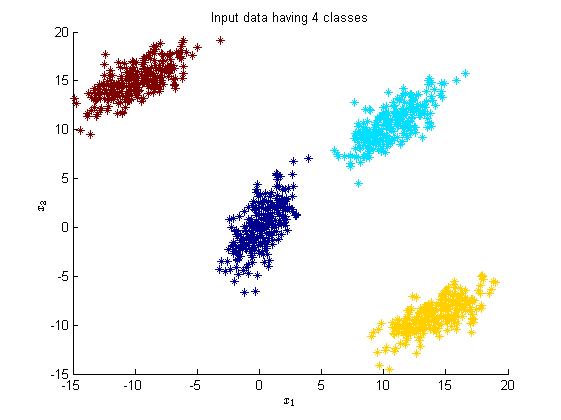
\includegraphics[width=\linewidth]{Classification/linearlySeparable/input_data.png}
\caption{Given dataset}
\end{figure}

\subsubsection{Linearly Separable Dataset}
\begin{flushleft}
In this dataset, we are given a 4 class problem, where every pair of classes is linearly separable. We are required to compare the performance of 3 classifiers mentioned above.
The input data is as shown in Figure 1. \\[10pt]

\textbf{Bayes Classifier :}  \\[10pt]

A Bayes classifier requires the estimation class conditional probability densities, for each class. We use a Gaussian Mixture Model for this purpose. We have assumed that the prior is same for each of the classes. Hence, the posterior probability of class is same as the class conditional density at any point.


From the plot, it's obvious that one Gaussian is sufficient to model each of class conditional densities.
Each of the densities were obtained by performing EM algorithm. 


The contours of each of the Gaussians obtained are shown in Figure 2. We can observe that the Gaussians model the distribution of points of each class correctly.



\begin{figure}[H]
\centering
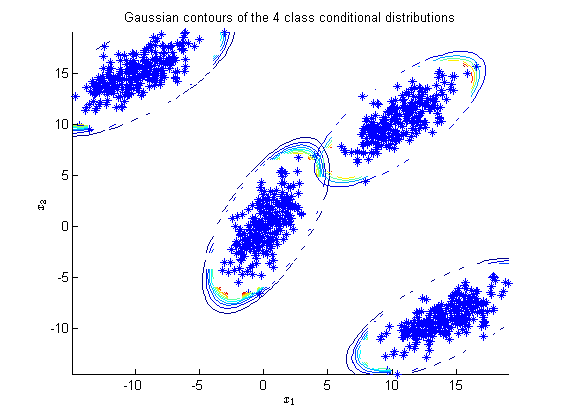
\includegraphics[width=\linewidth]{Classification/linearlySeparable/contours.png}
\caption{Given dataset}
\end{figure}

The results obtained are shown below in the form of confusion matrices :\\[10pt]

Train : \\[10pt]


\begin{tabular}{|c|c|}
\hline
150 & 0\\ 

\hline
0 & 600 \\ \hline

\end{tabular}\\[10pt]

Validation: \\[10pt]

\begin{tabular}{|c|c|} 
\hline
90 & 0\\ \hline
0 & 360 \\ \hline
\end{tabular}\\[10pt]

Test : \\[10pt]

\begin{tabular}{|c|c|} \hline 
60 & 0\\ \hline
0 & 240 \\ \hline 
 \end{tabular}\\[10pt]

We observe 100 \% accuracy in the classification of points in the validation and test data. The decision region plot, showing the separation between the 3 classes is shown in Figure 3.


\begin{figure}[H]
\centering
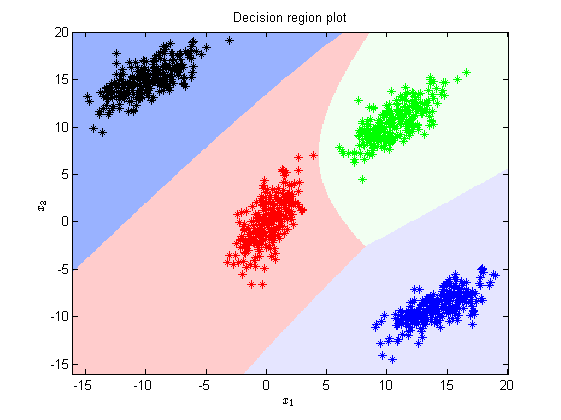
\includegraphics[width=\linewidth]{Classification/linearlySeparable/decn_region_bayes.png}
\caption{Given dataset}
\end{figure}


\end{flushleft}


\begin{flushleft}
\textbf{Perceptron Classifier :}  \\[10pt]

Since the data is linearly separable across pairs of classes, we can use the Perceptron model to classify the points. 

One approach is to use the One-Vs-All method for classification.  For the we require each of the 4 sets (using one class positive and others negative) to be linearly separable. If we consider the One-Vs-All classifier for the Red-Class (where point of red class are positive), we cannot find a separating hyperplane.

So, we use the approach of One-Vs-One classification.  $ 4 \choose 2 $ = 6 classifiers are constructed by considering each pair of classes. For any new point $x$, we use the outputs of each of the classifiers, and take the majority vote. As expected, the performance of training data was 100 \% as the hyperplane obtained separates the training data.  \\[10pt]

The results obtained are shown below  :\\[10pt]

\textbf{Train} : \\[10pt]


\begin{tabular}{|c|c|c|c|} \hline 250 & 0 & 0 & 0\\ \hline 0 & 250 & 0 & 0\\ \hline 0 & 0 & 250 & 0\\ \hline 0 & 0 & 0 & 250 \\ \hline \end{tabular} \\[10pt]

\textbf{Validation} : \\[10pt]

\begin{tabular}{|c|c|c|c|}  \hline 149 & 0 & 0 & 1\\ \hline 0 & 150 & 0 & 0\\ \hline 0 & 0 & 150 & 0\\ \hline 0 & 0 & 0 & 150 \\ \hline \end{tabular}  \\[10pt]


\textbf{Test}: \\[10pt]


\begin{tabular}{|c|c|c|c|}\hline 100 & 0 & 0 & 0\\ \hline 1 & 99 & 0 & 0\\ \hline 0 & 0 & 100 & 0\\ \hline 0 & 0 & 0 & 100 \\ \hline \end{tabular} \\[10pt]



From the results, we see that only one point is misclassified in the validation and test datasets, and that one point is a point in class 1 which is misclassified as class 2. This is because both the classes are very close to each other, and the hyperplanes obtained are not the optimal ones. \\[10pt]

The decision region plot obtained, showing the separation between the 3 classes is shown in Figure 4.


\begin{figure}[H]
\centering
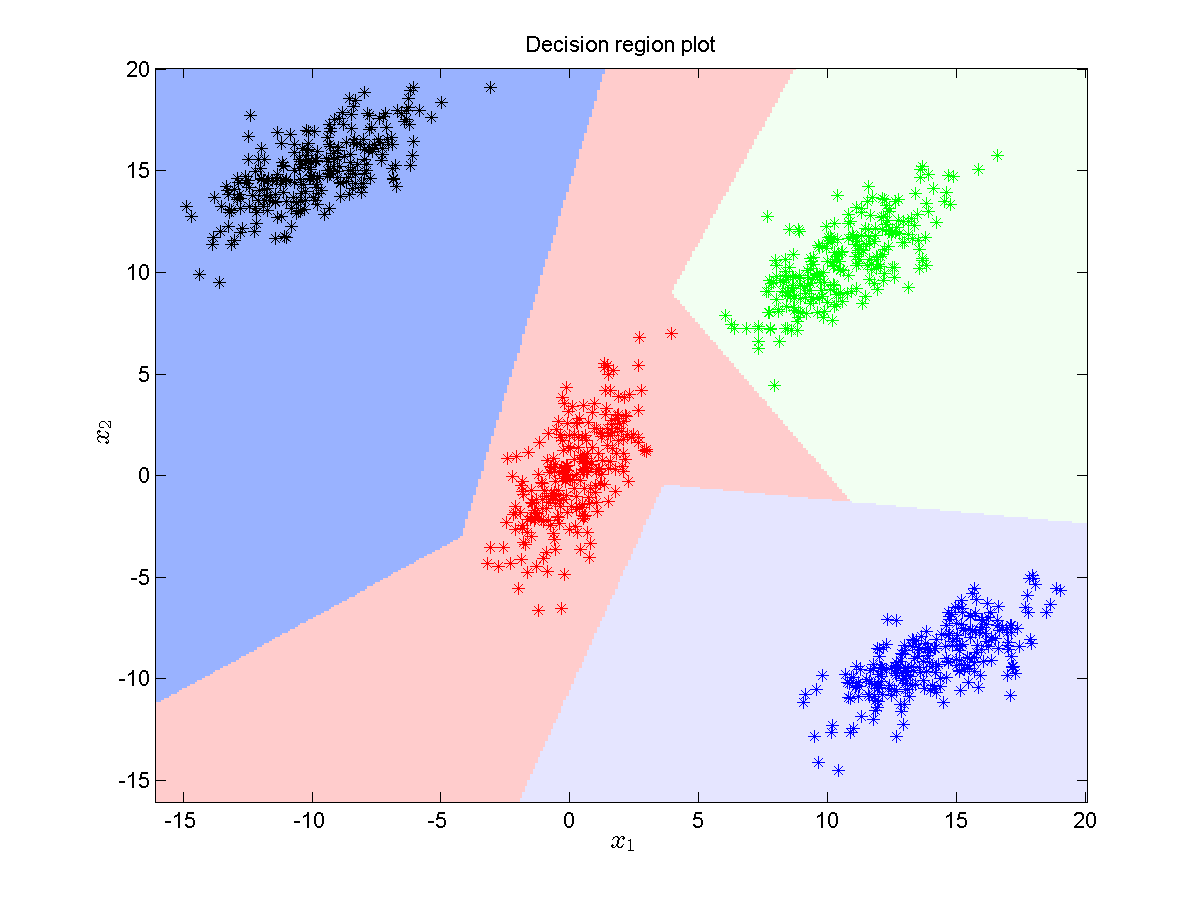
\includegraphics[width=\linewidth]{Classification/linearlySeparable/decn_region_perceptron.png}
\caption{}
\end{figure}
\newpage
\textbf{MLFFNN :} \\[10pt]

For this simple dataset, we use a feedforward neural network with 1 hidden layer. There are 4 nodes in the output layer, for which we use a 1-of-k representation of the class labels. The function used is the one available in the MATLAB \textit{nntools} toolbox. The MSE error function was used in the output layer.
The number of nodes in the hidden layer (model complexity) was estimated to be 9 with hyperbolic tangent function, using multiple iterations of cross-validation. For this configuration, the results obtained are shown below :
	
% Confusion matrices %
\textbf{\\[5pt]Confusion Matrices: \\[10pt]}
\textbf{Train :\\[5pt]}

\begin{tabular}{|c|c|c|c|} \hline 250 & 0 & 0 & 0\\ \hline 0 & 250 & 0 & 0\\ \hline 0 & 0 & 250 & 0\\ \hline 0 & 0 & 0 & 250 \\ \hline \end{tabular}


\textbf{\\[10pt]Validation :\\[5pt]}

\begin{tabular}{|c|c|c|c|c|} \hline  0 & 0 & 0 & 150\\ \hline 150 & 0 & 0 & 0\\ \hline 0 & 150 & 0 & 0\\ \hline  0 & 0 & 150 & 0\\ \hline 0 & 0 & 0 & 0 \\ \hline \end{tabular}

\textbf{\\[10pt]Test :\\[5pt]}


\begin{tabular}{|c|c|c|c|} \hline 100 & 0 & 0 & 0\\ \hline 0 & 100 & 0 & 0\\ \hline 0 & 0 & 100 & 0\\ \hline 0 & 0 & 0 & 100 \\ \hline \end{tabular}




\textbf{\\[10pt]Decision Region:\\[5pt]}
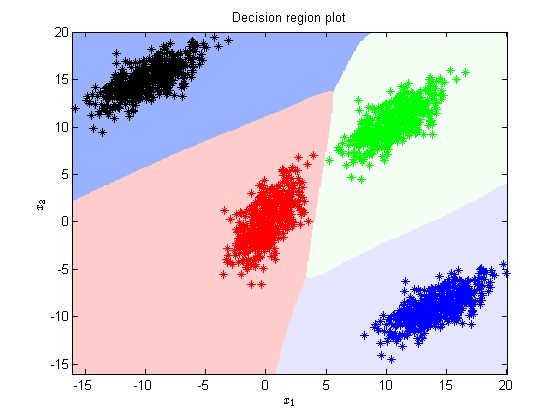
\includegraphics[scale=1]{Classification/linearlySeparable/decn_region_nn}

\textbf{\\[10pt]Output Layer Plots across Epochs of training}
\begin{figure}
\begin{subfigure}{.5\textwidth}
  \centering
  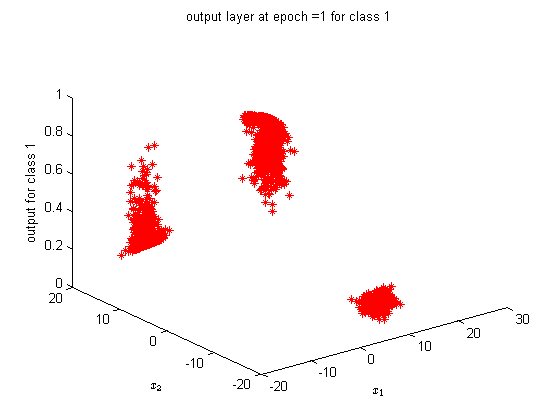
\includegraphics[width=.8\linewidth]{Classification/linearlySeparable/1_1}
 
\end{subfigure}%
\begin{subfigure}{.5\textwidth}
  \centering
  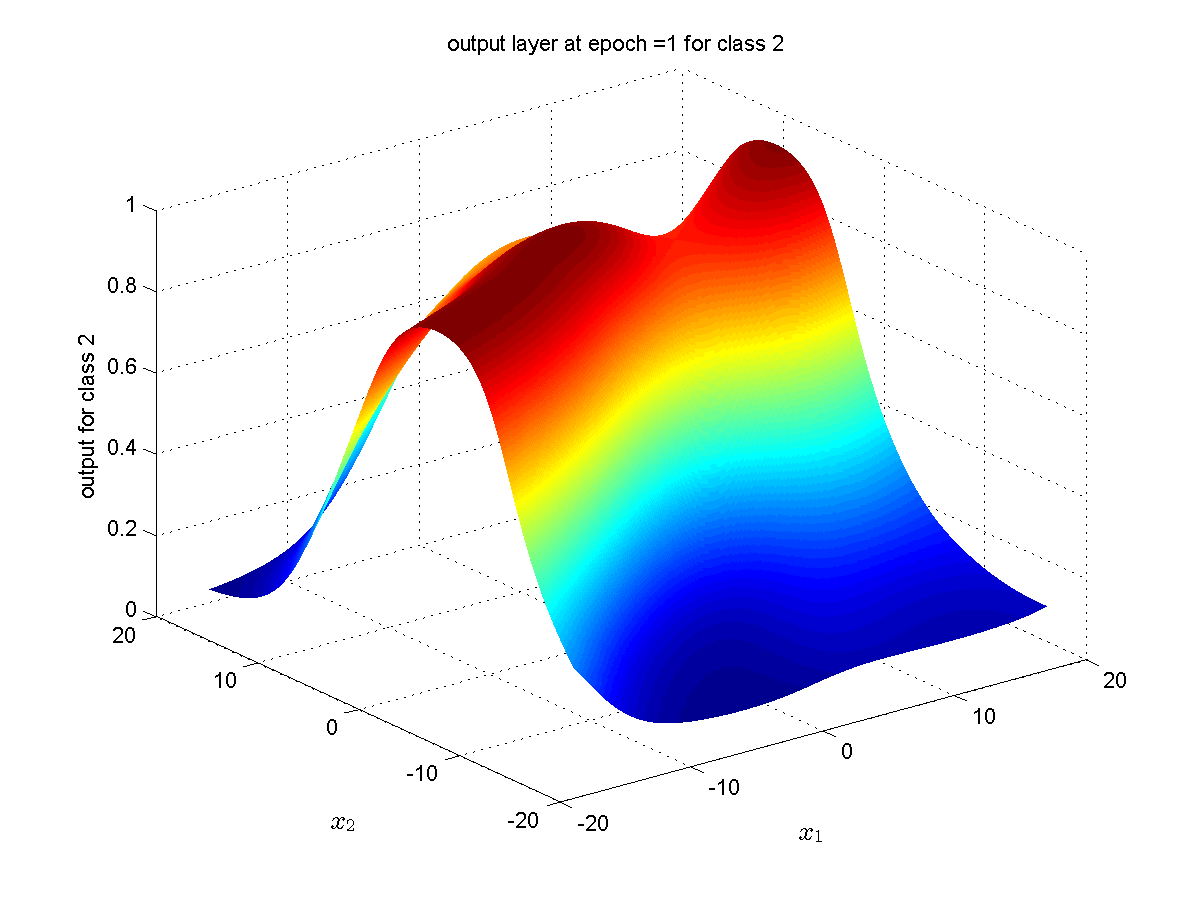
\includegraphics[width=.8\linewidth]{Classification/linearlySeparable/1_2}
  
\end{subfigure}
\caption{Epoch 1 class 1 and 2}
\end{figure}

\begin{figure}
\begin{subfigure}{.5\textwidth}
  \centering
  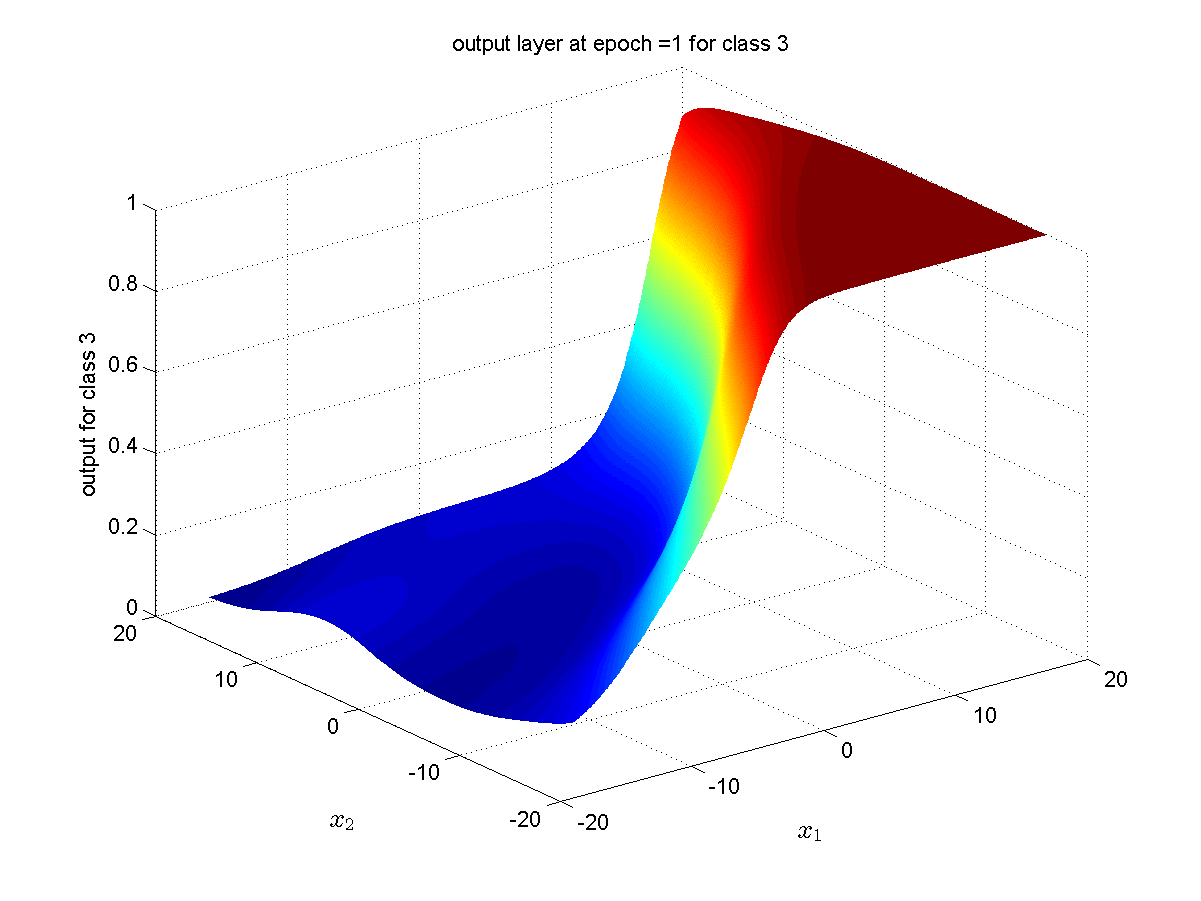
\includegraphics[width=.8\linewidth]{Classification/linearlySeparable/1_3}
 
\end{subfigure}%
\begin{subfigure}{.5\textwidth}
  \centering
  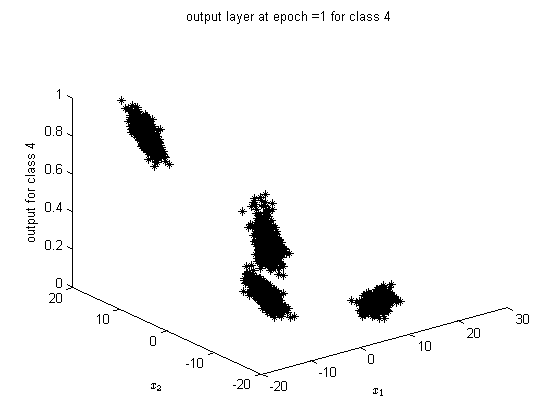
\includegraphics[width=.8\linewidth]{Classification/linearlySeparable/1_4}
  
\end{subfigure}
\caption{Epoch 1 class 3 and 4}
\end{figure}

\begin{figure}
\begin{subfigure}{.5\textwidth}
  \centering
  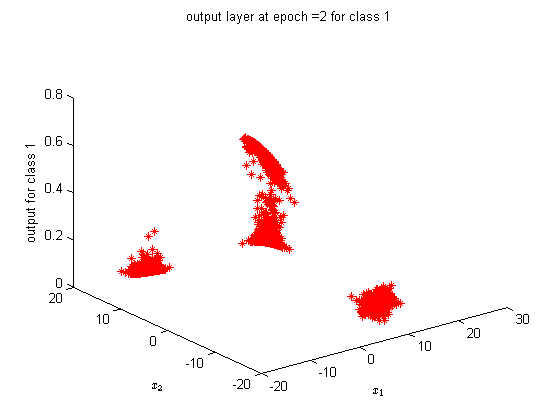
\includegraphics[width=.8\linewidth]{Classification/linearlySeparable/2_1}
 
\end{subfigure}%
\begin{subfigure}{.5\textwidth}
  \centering
  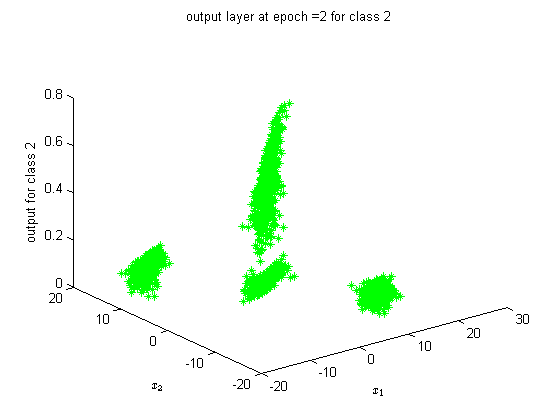
\includegraphics[width=.8\linewidth]{Classification/linearlySeparable/2_2}
  
\end{subfigure}
\caption{Epoch 2 class 1 and 2}
\end{figure}

\begin{figure}
\begin{subfigure}{.5\textwidth}
  \centering
  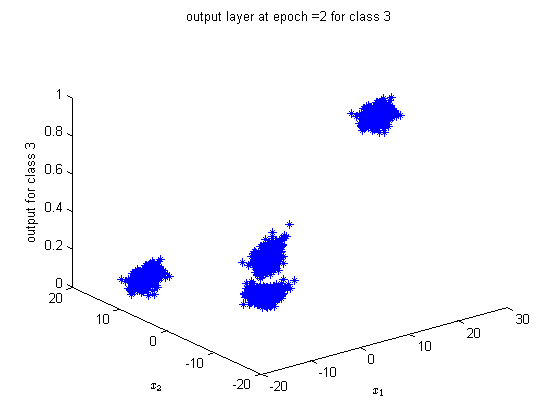
\includegraphics[width=.8\linewidth]{Classification/linearlySeparable/2_3}
 
\end{subfigure}%
\begin{subfigure}{.5\textwidth}
  \centering
  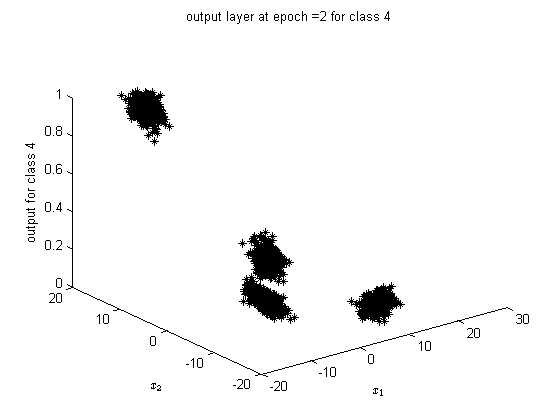
\includegraphics[width=.8\linewidth]{Classification/linearlySeparable/2_4}
  
\end{subfigure}
\caption{Epoch 2 class 3 and 4}
\end{figure}

\begin{figure}
\begin{subfigure}{.5\textwidth}
  \centering
  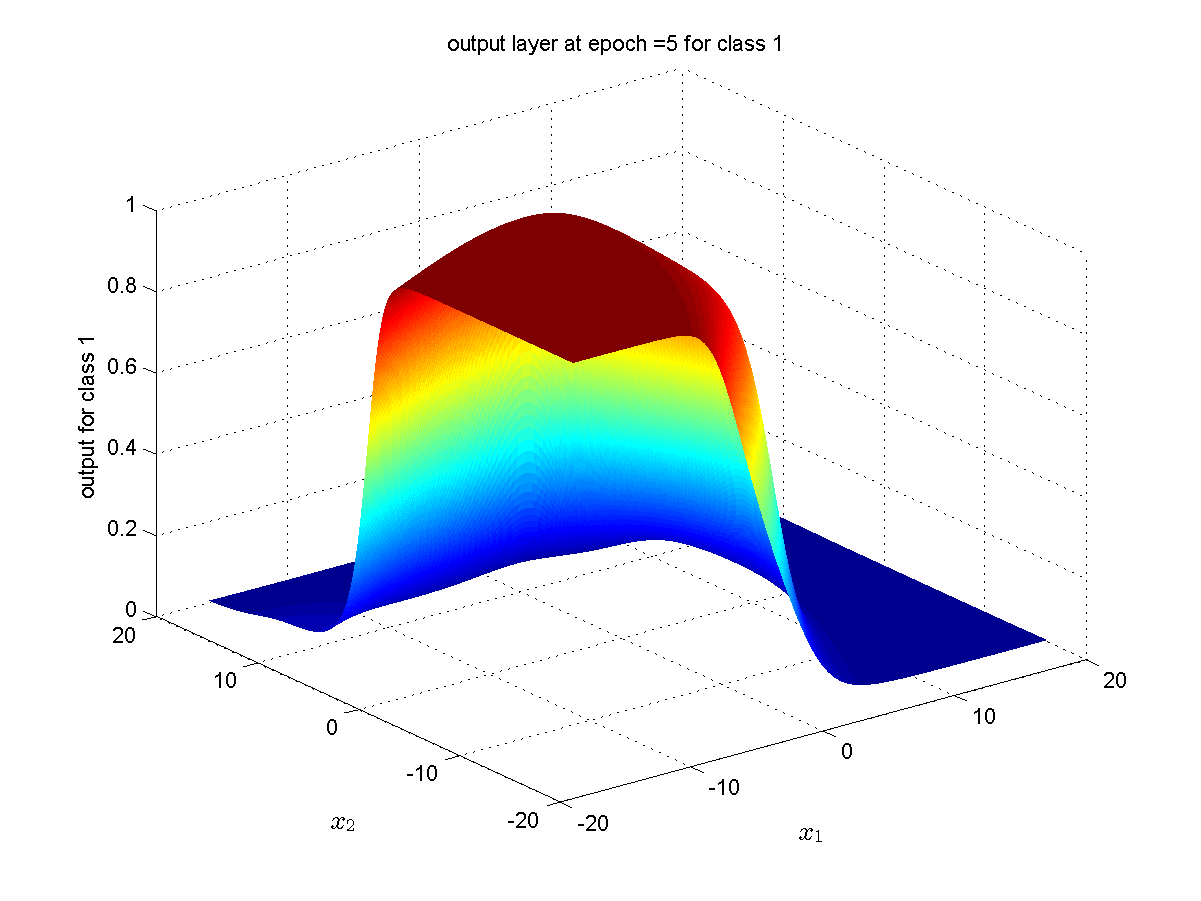
\includegraphics[width=.8\linewidth]{Classification/linearlySeparable/5_1}
 
\end{subfigure}%
\begin{subfigure}{.5\textwidth}
  \centering
  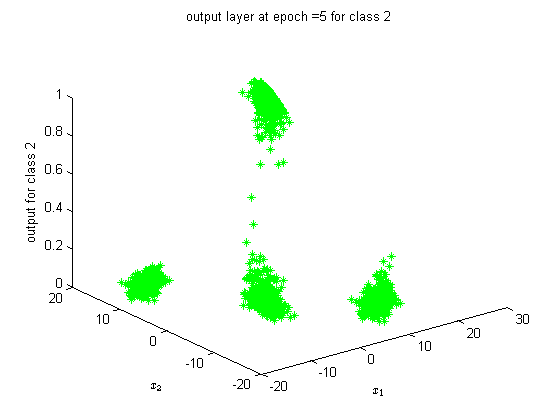
\includegraphics[width=.8\linewidth]{Classification/linearlySeparable/5_2}
  
\end{subfigure}
\caption{Epoch 5 class 1 and 2}
\end{figure}

\begin{figure}
\begin{subfigure}{.5\textwidth}
  \centering
  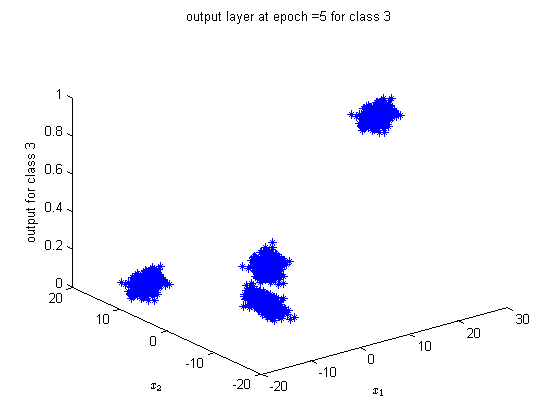
\includegraphics[width=.8\linewidth]{Classification/linearlySeparable/5_3}
 
\end{subfigure}%
\begin{subfigure}{.5\textwidth}
  \centering
  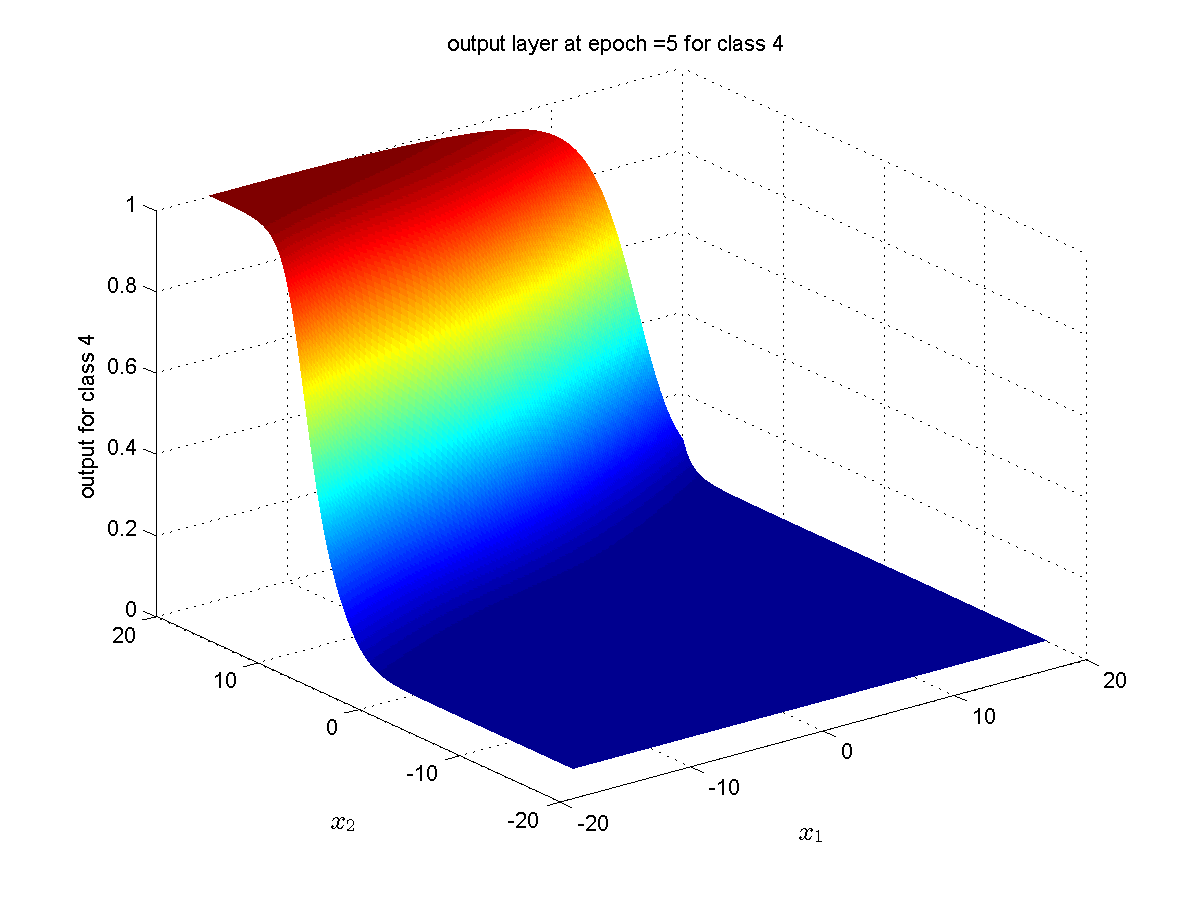
\includegraphics[width=.8\linewidth]{Classification/linearlySeparable/5_4}
  
\end{subfigure}
\caption{Epoch 5 class 3 and 4}
\end{figure}


\begin{figure}
\begin{subfigure}{.5\textwidth}
  \centering
  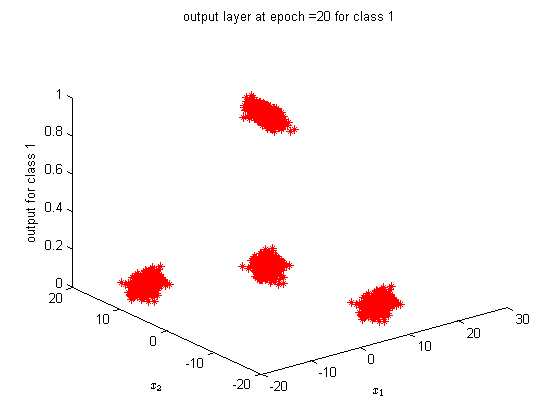
\includegraphics[width=.8\linewidth]{Classification/linearlySeparable/20_1}
 
\end{subfigure}%
\begin{subfigure}{.5\textwidth}
  \centering
  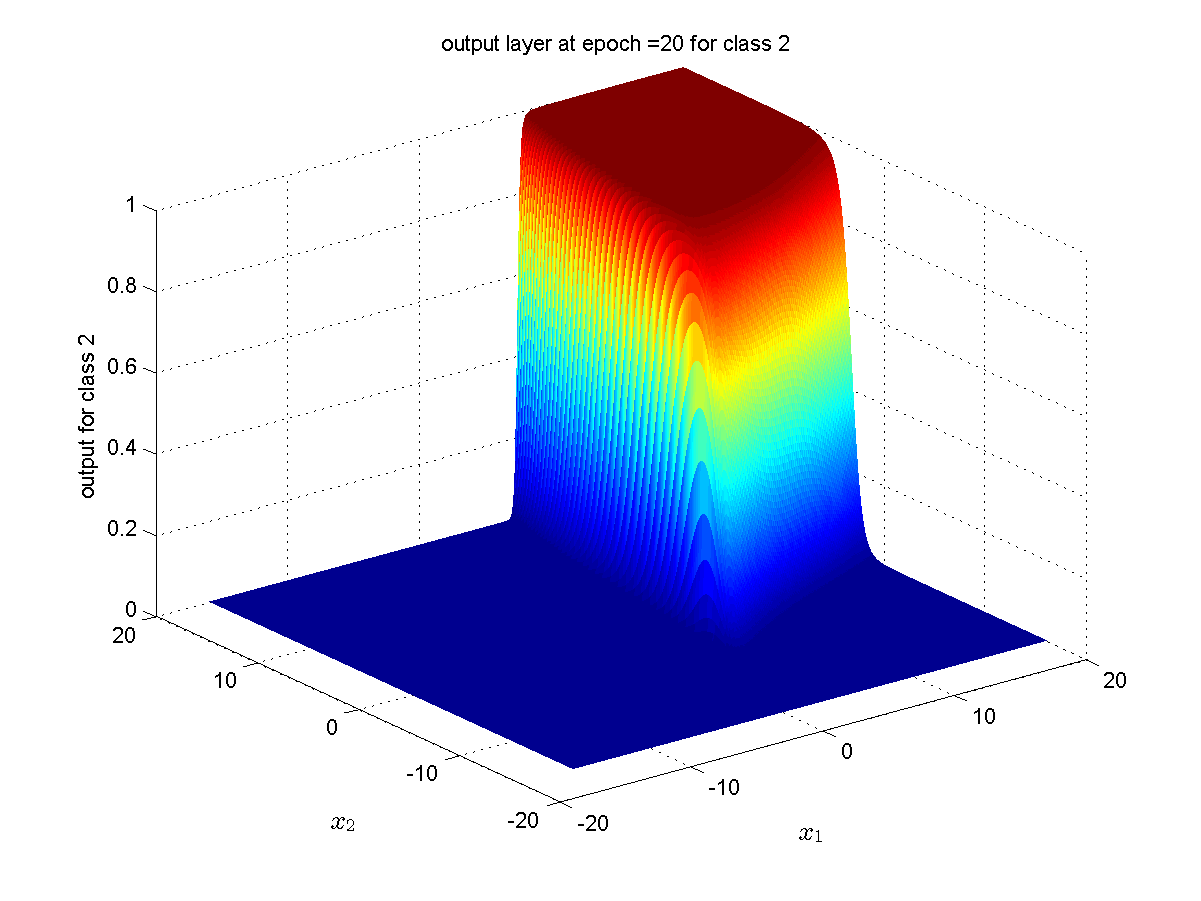
\includegraphics[width=.8\linewidth]{Classification/linearlySeparable/20_2}
  
\end{subfigure}
\caption{Epoch 20 class 1 and 2}
\end{figure}

\begin{figure}
\begin{subfigure}{.5\textwidth}
  \centering
  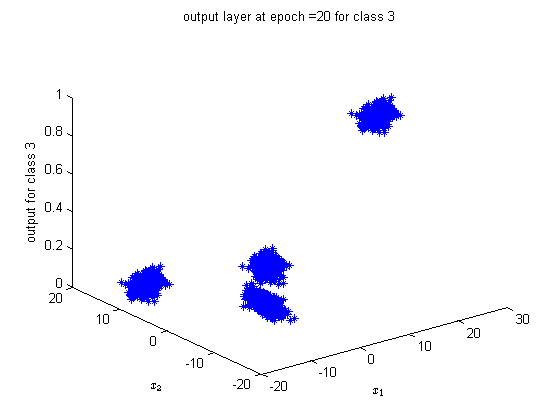
\includegraphics[width=.8\linewidth]{Classification/linearlySeparable/20_3}
 
\end{subfigure}%
\begin{subfigure}{.5\textwidth}
  \centering
  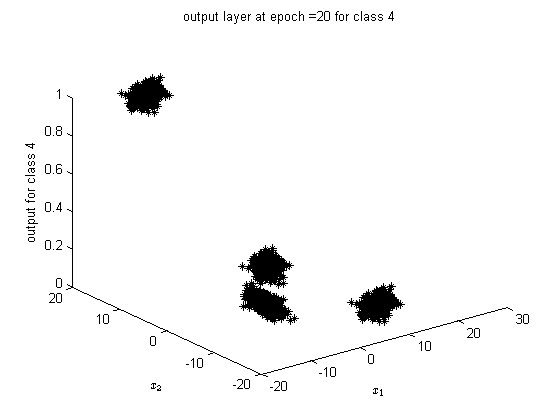
\includegraphics[width=.8\linewidth]{Classification/linearlySeparable/20_4}
  
\end{subfigure}
\caption{Epoch 20 class 3 and 4}
\end{figure}
Clearly, a stable output has been established by the 20th epoch, looking at the above plots. We also proceed to look at what the hidden layer is outputing at some epochs. \\[10pt]
\begin{figure}
\begin{subfigure}{.3\textwidth}
  \centering
  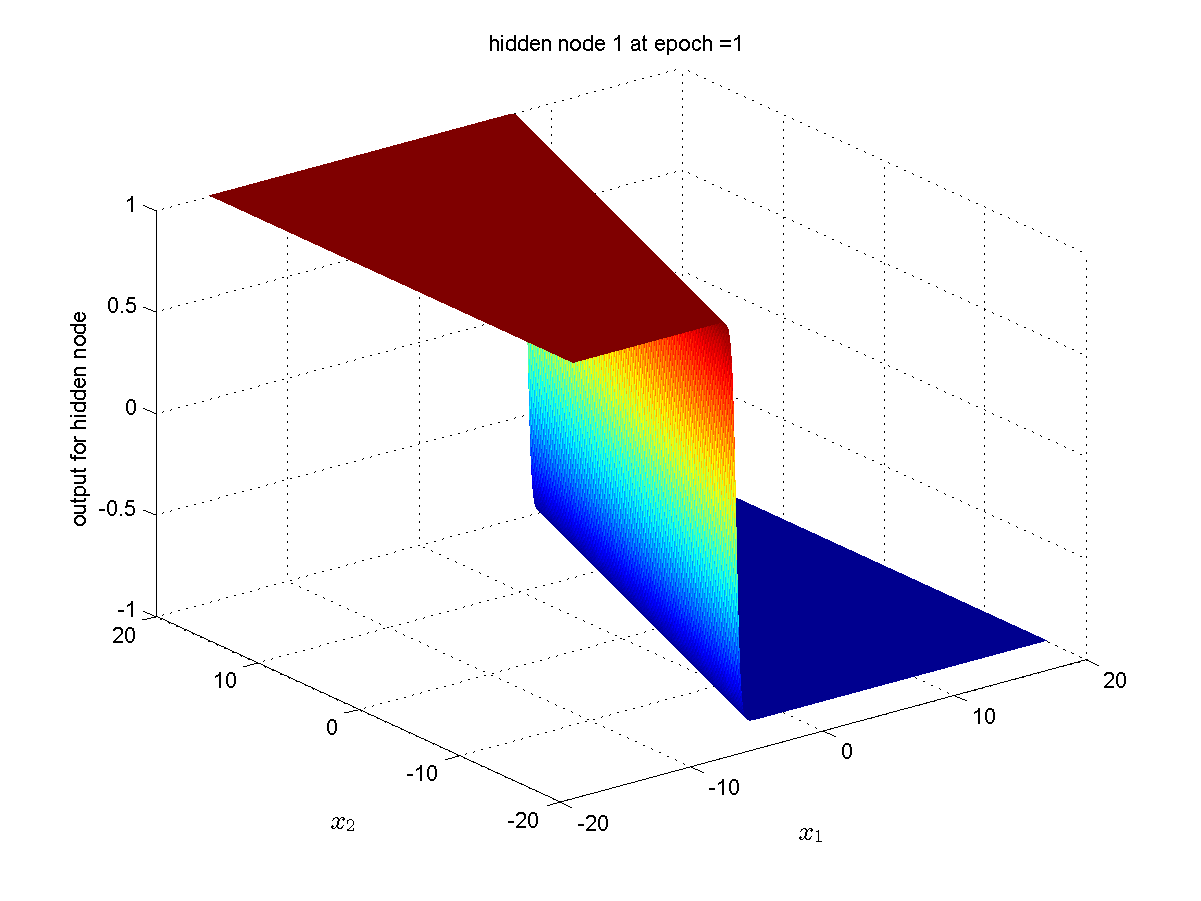
\includegraphics[width=.8\linewidth]{Classification/linearlySeparable/h1_1}
 
\end{subfigure}%
\begin{subfigure}{.3\textwidth}
  \centering
  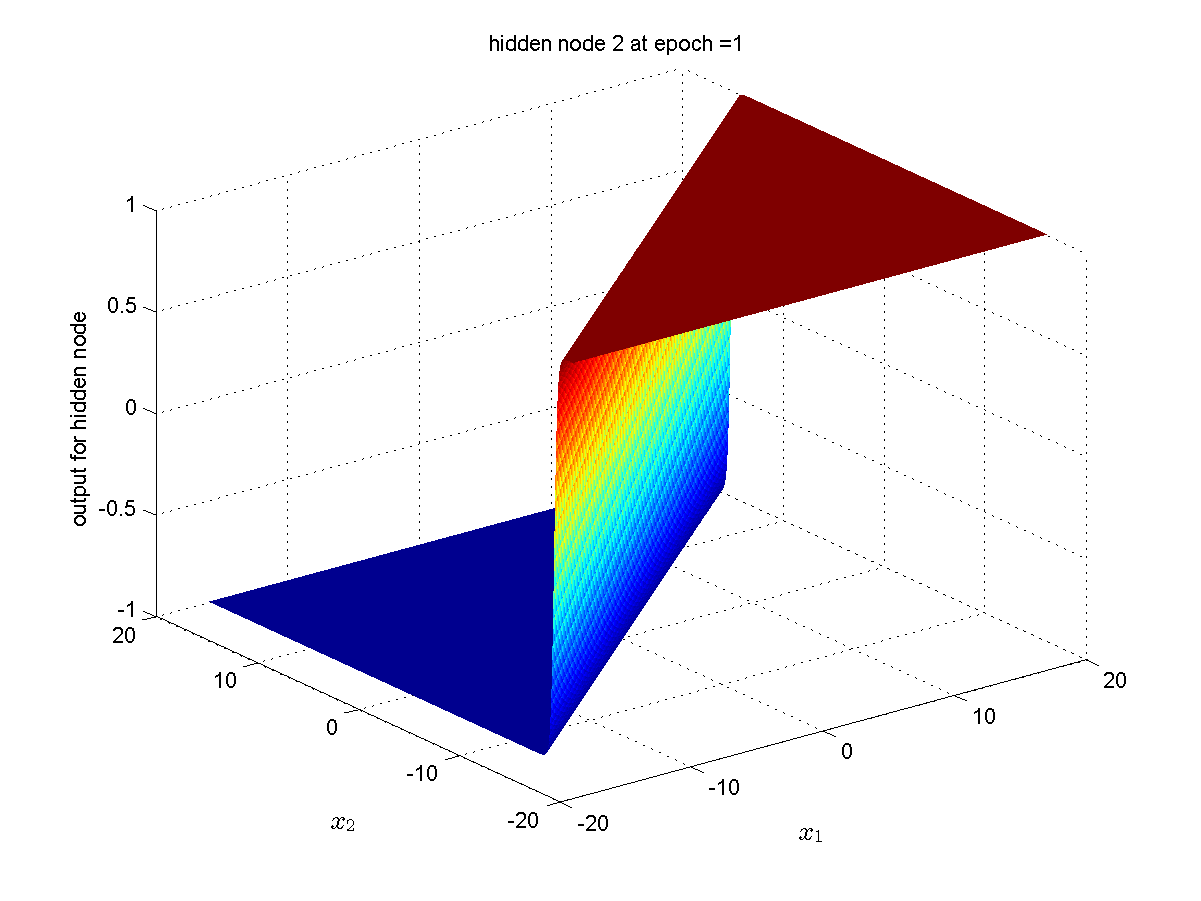
\includegraphics[width=.8\linewidth]{Classification/linearlySeparable/h1_2}
  
\end{subfigure}
\begin{subfigure}{.3\textwidth}
  \centering
  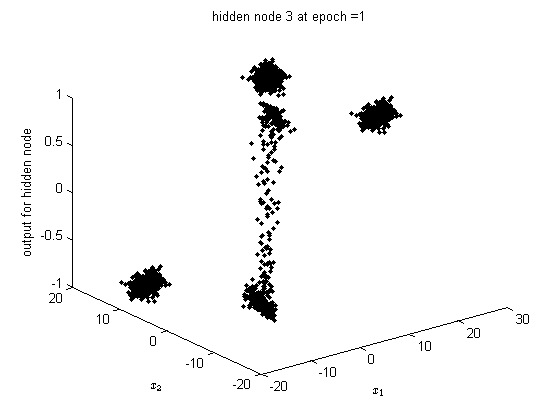
\includegraphics[width=.8\linewidth]{Classification/linearlySeparable/h1_3}
  
\end{subfigure}
\caption{Epoch 1 hidden nodes 1,2,3}
\end{figure}

\begin{figure}
\begin{subfigure}{.3\textwidth}
  \centering
  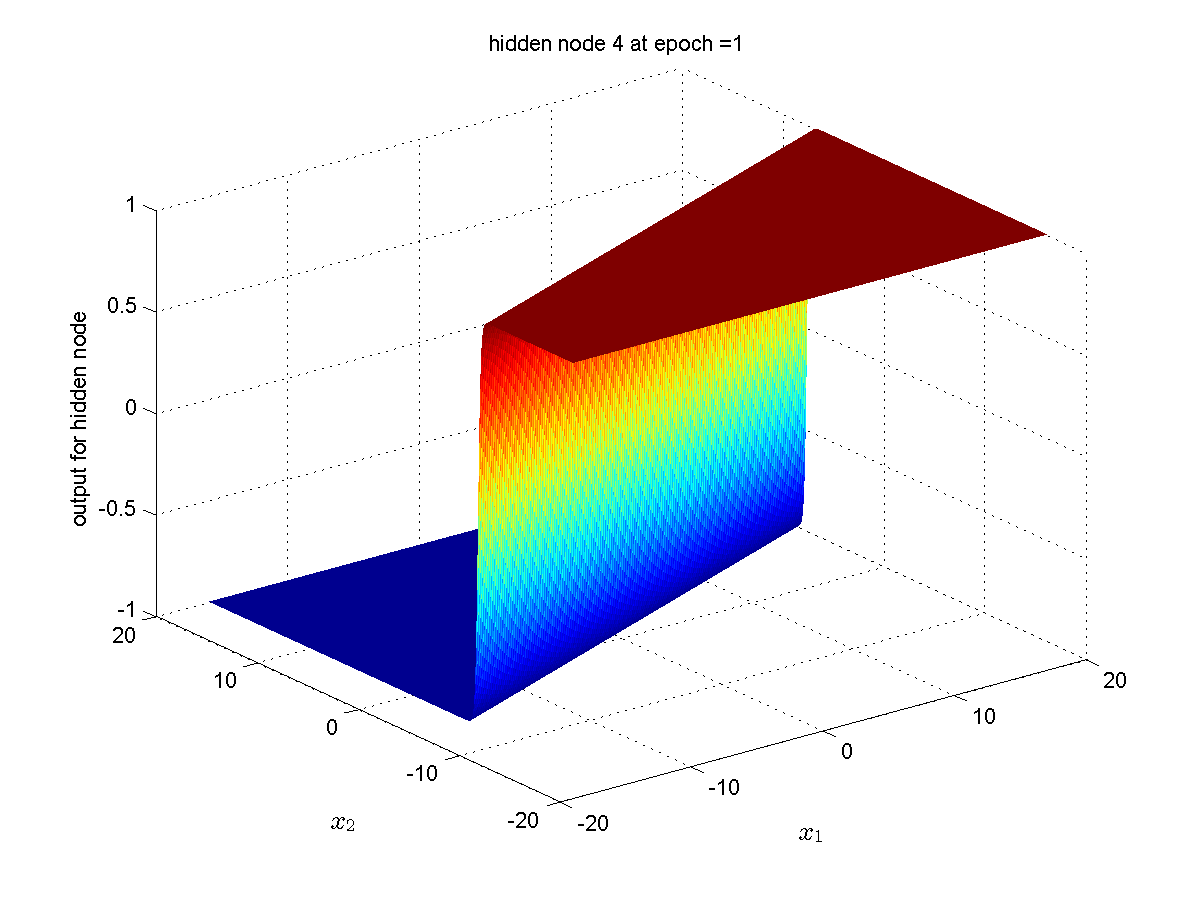
\includegraphics[width=.8\linewidth]{Classification/linearlySeparable/h1_4}
 
\end{subfigure}%
\begin{subfigure}{.3\textwidth}
  \centering
  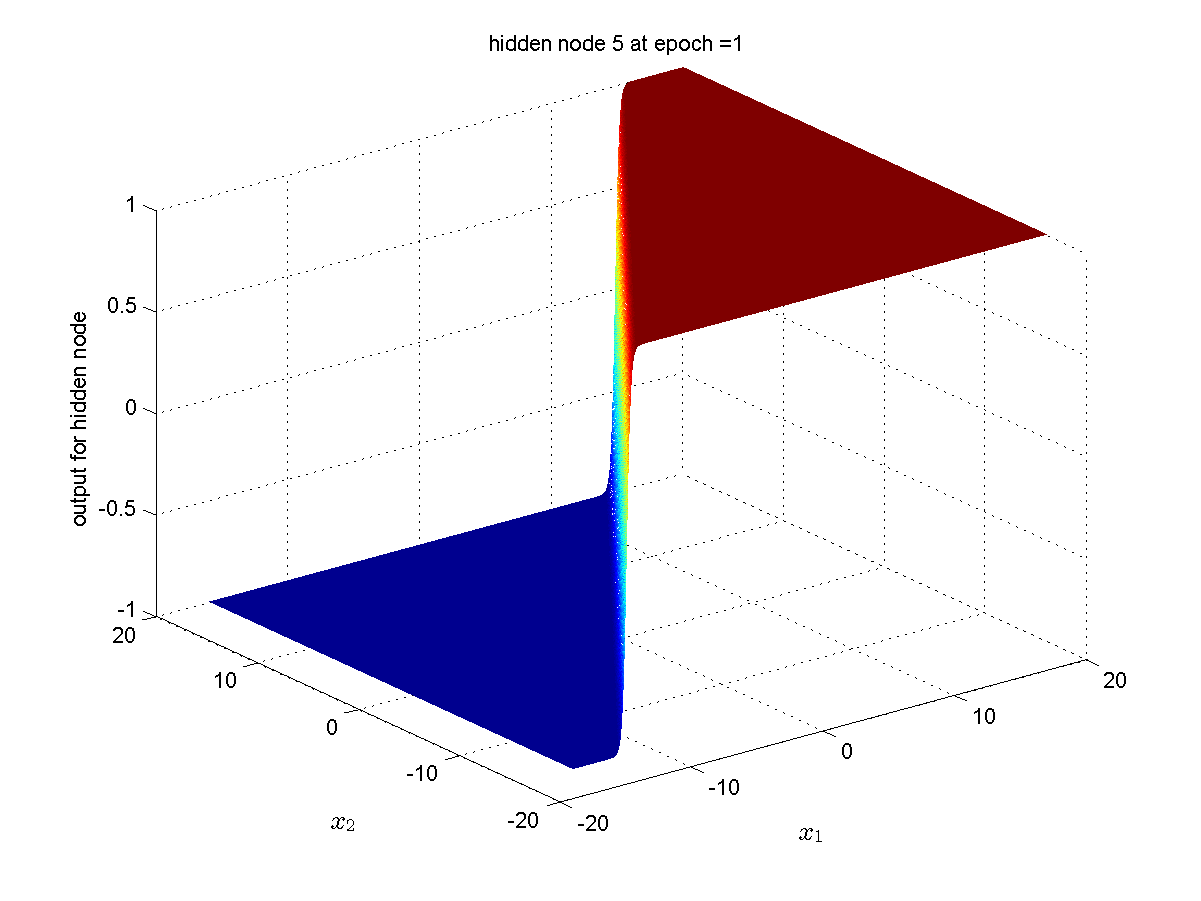
\includegraphics[width=.8\linewidth]{Classification/linearlySeparable/h1_5}
  
\end{subfigure}
\begin{subfigure}{.3\textwidth}
  \centering
  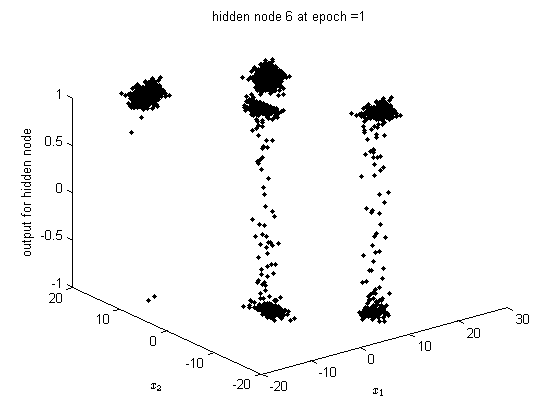
\includegraphics[width=.8\linewidth]{Classification/linearlySeparable/h1_6}
  
\end{subfigure}
\caption{Epoch 1 hidden nodes 4,5,6}
\end{figure}

\begin{figure}
\begin{subfigure}{.3\textwidth}
  \centering
  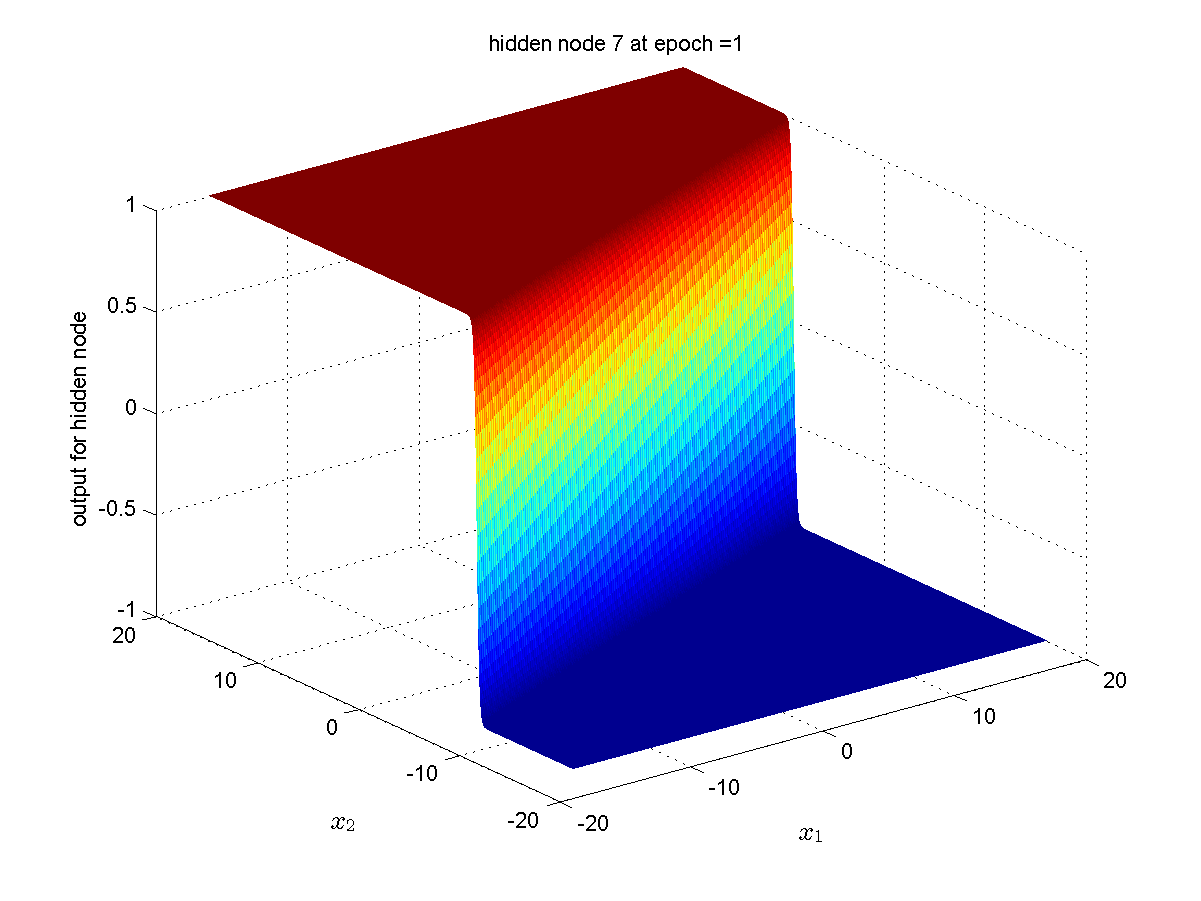
\includegraphics[width=.8\linewidth]{Classification/linearlySeparable/h1_7}
 
\end{subfigure}%
\begin{subfigure}{.3\textwidth}
  \centering
  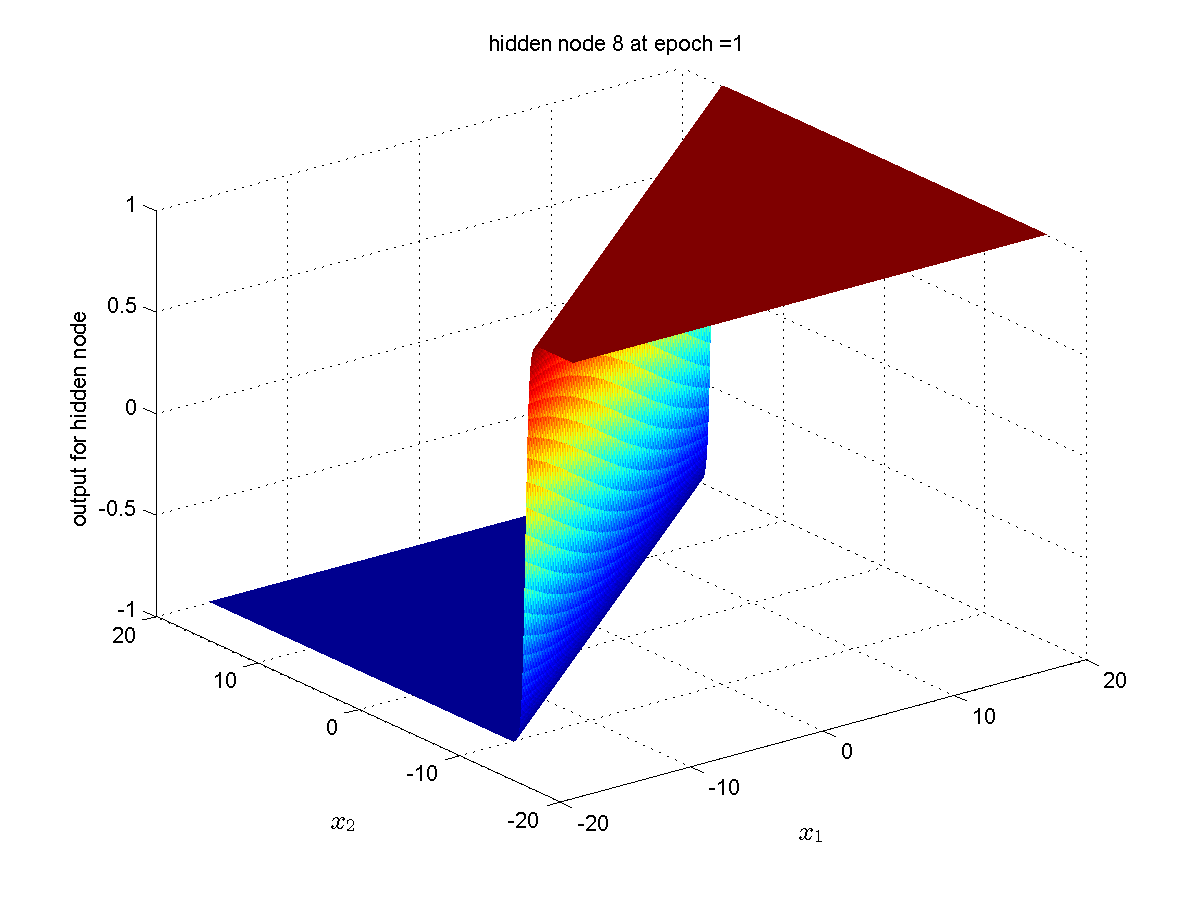
\includegraphics[width=.8\linewidth]{Classification/linearlySeparable/h1_8}
  
\end{subfigure}
\begin{subfigure}{.3\textwidth}
  \centering
  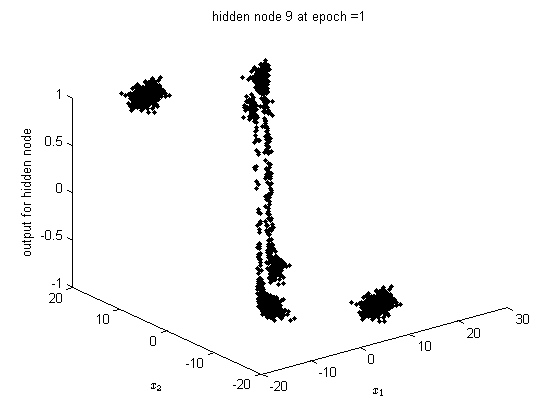
\includegraphics[width=.8\linewidth]{Classification/linearlySeparable/h1_9}
  
\end{subfigure}
\caption{Epoch 1 hidden nodes 7,8,9}
\end{figure}

\newpage
\begin{figure}
\begin{subfigure}{.3\textwidth}
  \centering
  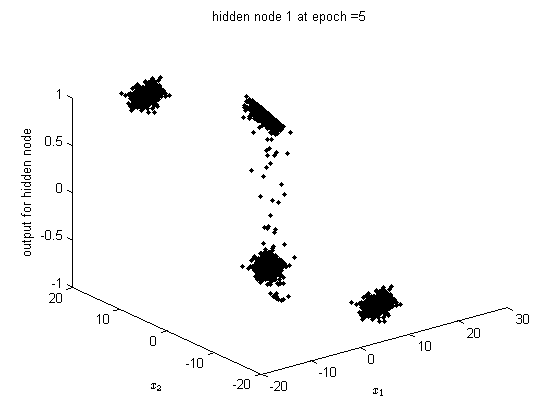
\includegraphics[width=.8\linewidth]{Classification/linearlySeparable/h5_1}
 
\end{subfigure}%
\begin{subfigure}{.3\textwidth}
  \centering
  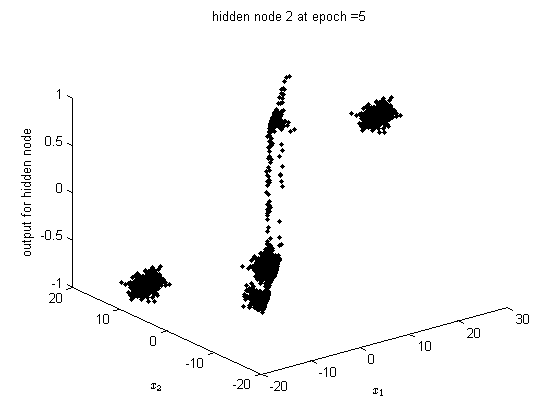
\includegraphics[width=.8\linewidth]{Classification/linearlySeparable/h5_2}
  
\end{subfigure}
\begin{subfigure}{.3\textwidth}
  \centering
  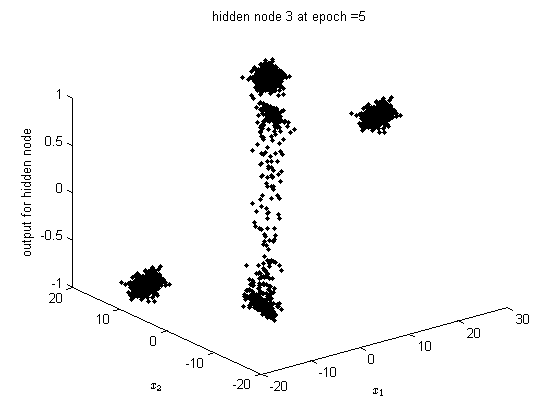
\includegraphics[width=.8\linewidth]{Classification/linearlySeparable/h5_3}
  
\end{subfigure}
\caption{Epoch 5 hidden nodes 1,2,3}
\end{figure}

\begin{figure}
\begin{subfigure}{.3\textwidth}
  \centering
  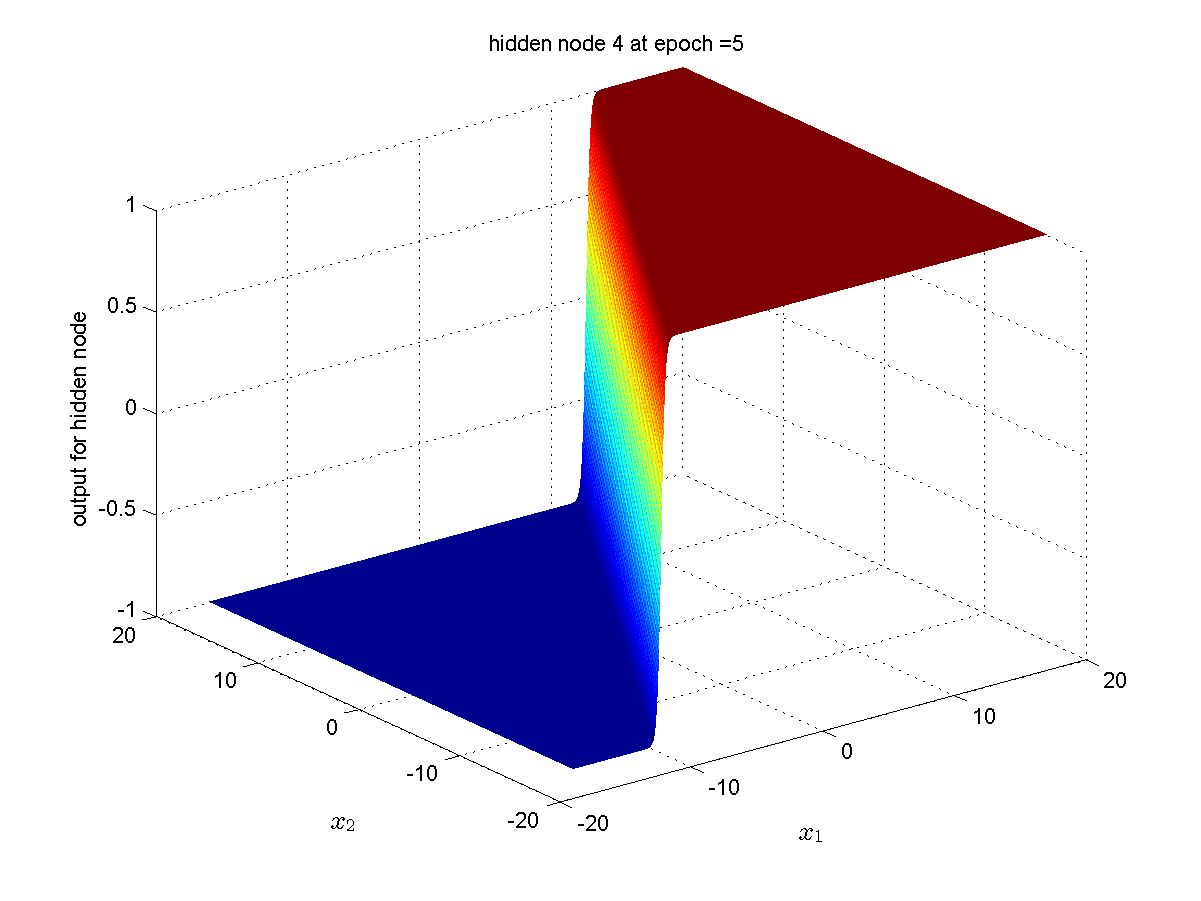
\includegraphics[width=.8\linewidth]{Classification/linearlySeparable/h5_4}
 
\end{subfigure}%
\begin{subfigure}{.3\textwidth}
  \centering
  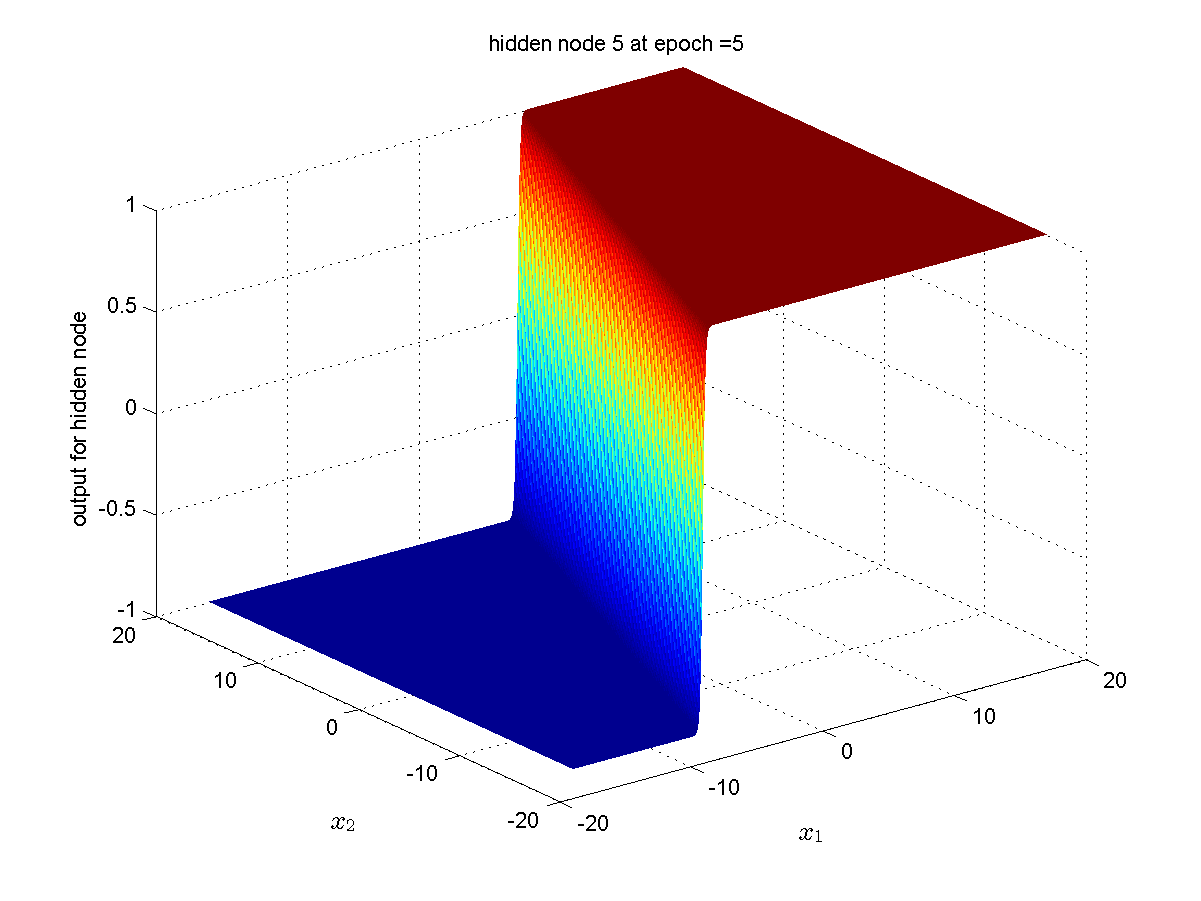
\includegraphics[width=.8\linewidth]{Classification/linearlySeparable/h5_5}
  
\end{subfigure}
\begin{subfigure}{.3\textwidth}
  \centering
  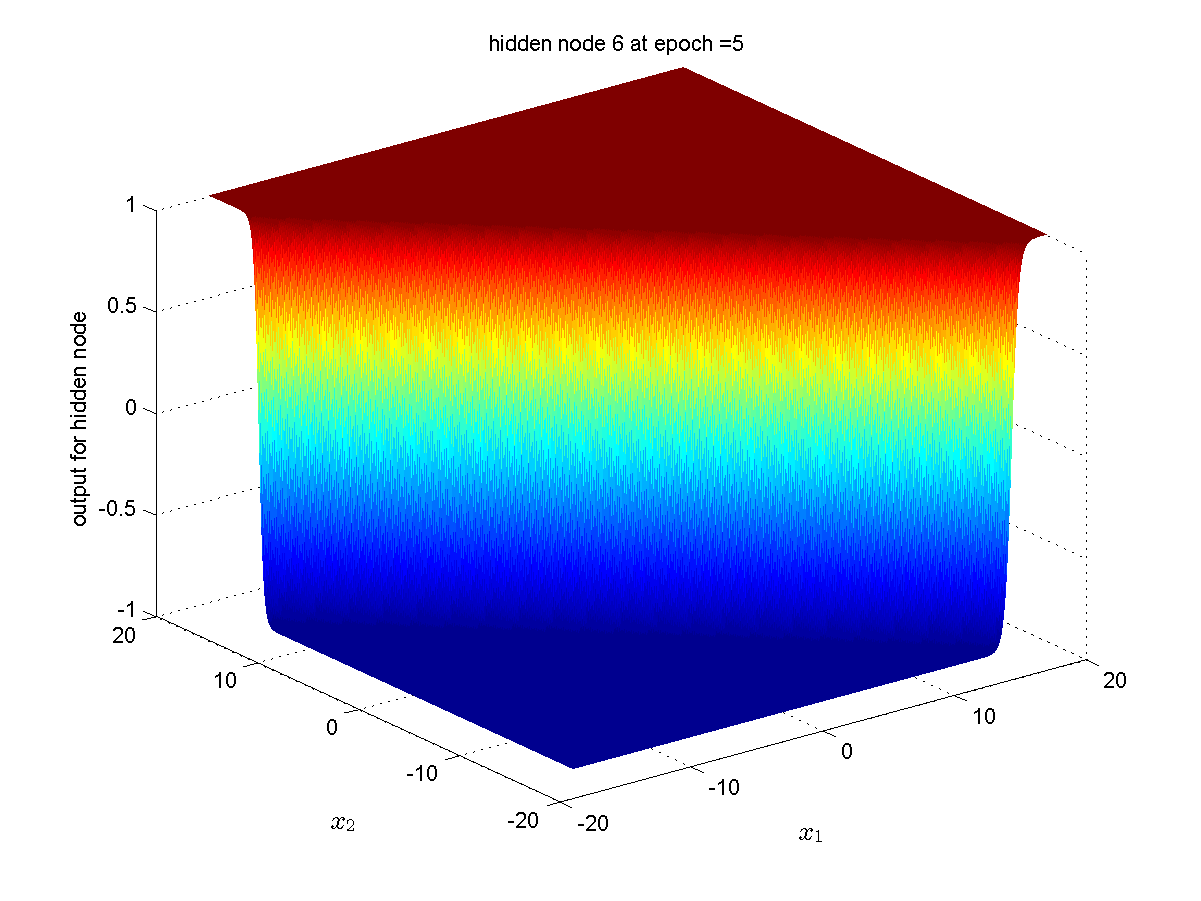
\includegraphics[width=.8\linewidth]{Classification/linearlySeparable/h5_6}
  
\end{subfigure}
\caption{Epoch 5 hidden nodes 4,5,6}
\end{figure}

\begin{figure}
\begin{subfigure}{.3\textwidth}
  \centering
  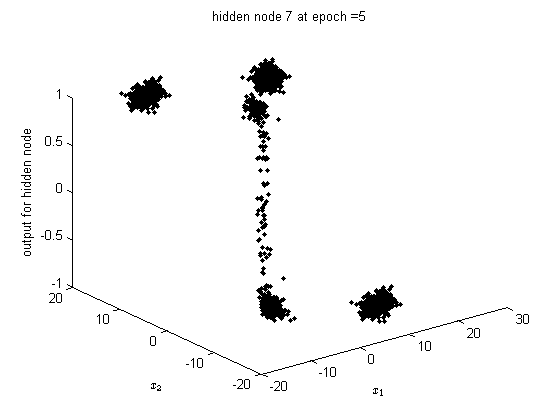
\includegraphics[width=.8\linewidth]{Classification/linearlySeparable/h5_7}
 
\end{subfigure}%
\begin{subfigure}{.3\textwidth}
  \centering
  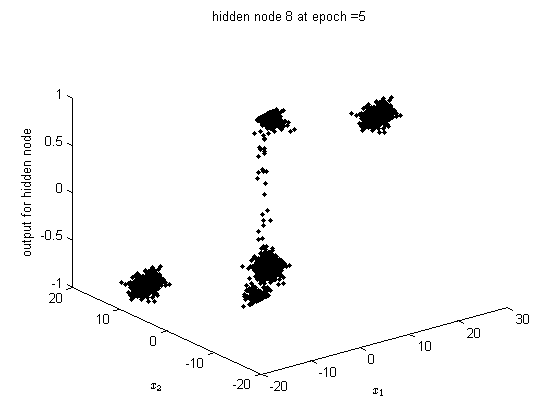
\includegraphics[width=.8\linewidth]{Classification/linearlySeparable/h5_8}
  
\end{subfigure}
\begin{subfigure}{.3\textwidth}
  \centering
  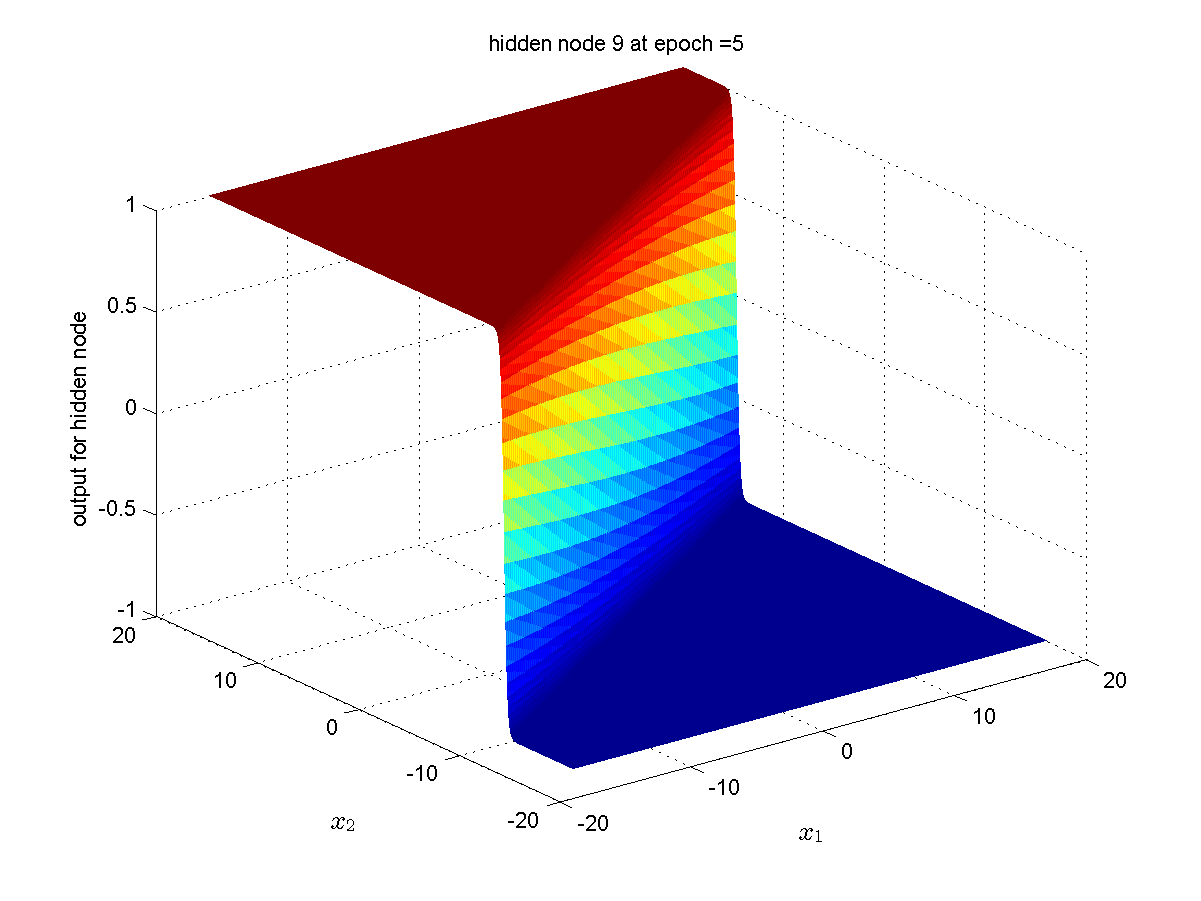
\includegraphics[width=.8\linewidth]{Classification/linearlySeparable/h5_9}
  
\end{subfigure}
\caption{Epoch 5 hidden nodes 7,8,9}
\end{figure}
\newpage
\begin{figure}
\begin{subfigure}{.3\textwidth}
  \centering
  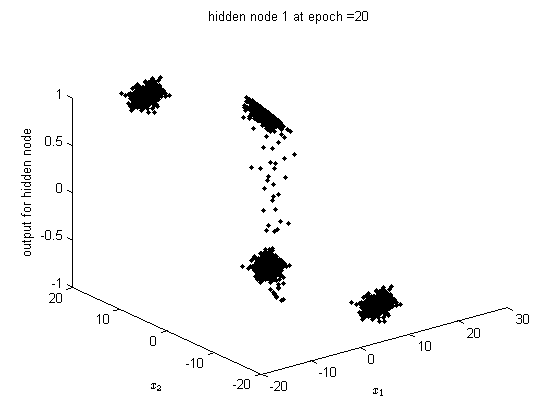
\includegraphics[width=.8\linewidth]{Classification/linearlySeparable/h20_1}
 
\end{subfigure}%
\begin{subfigure}{.3\textwidth}
  \centering
  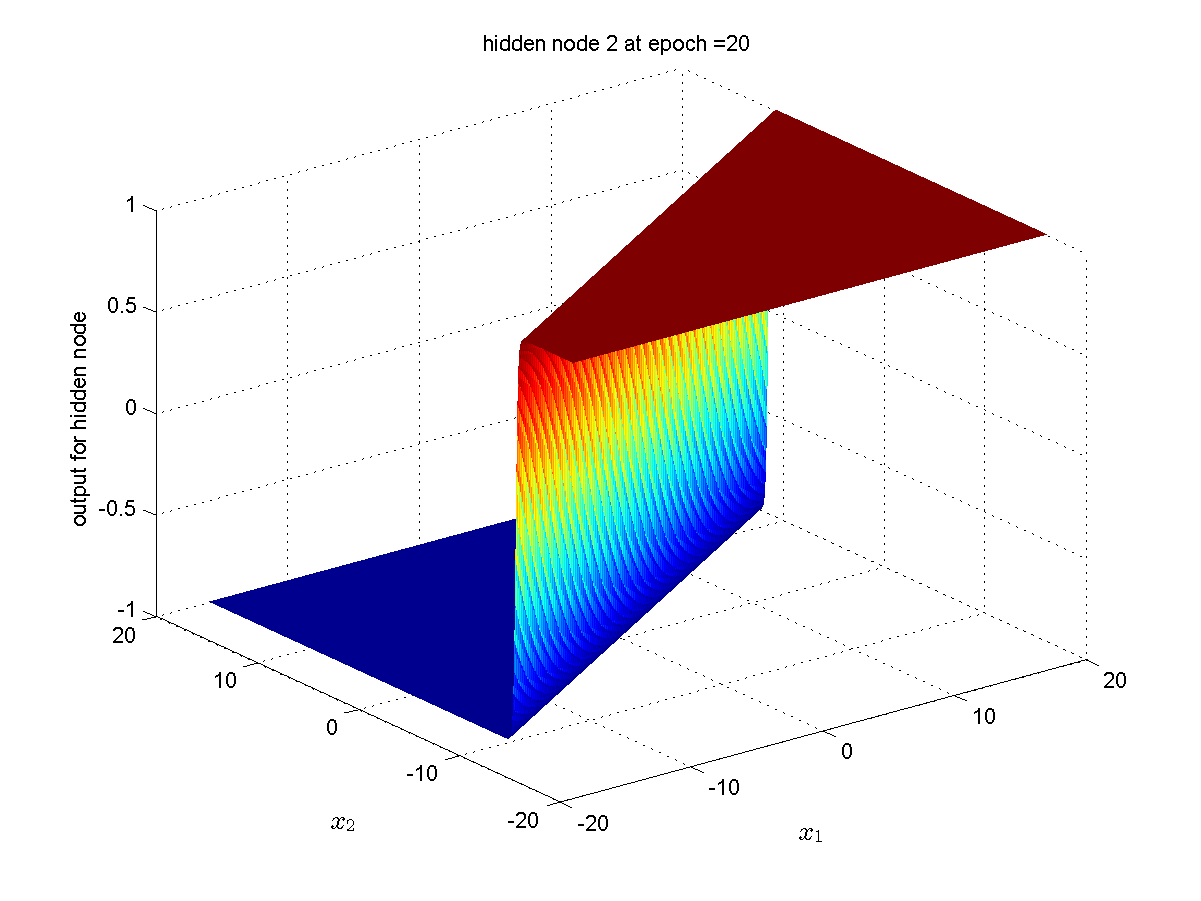
\includegraphics[width=.8\linewidth]{Classification/linearlySeparable/h20_2}
  
\end{subfigure}
\begin{subfigure}{.3\textwidth}
  \centering
  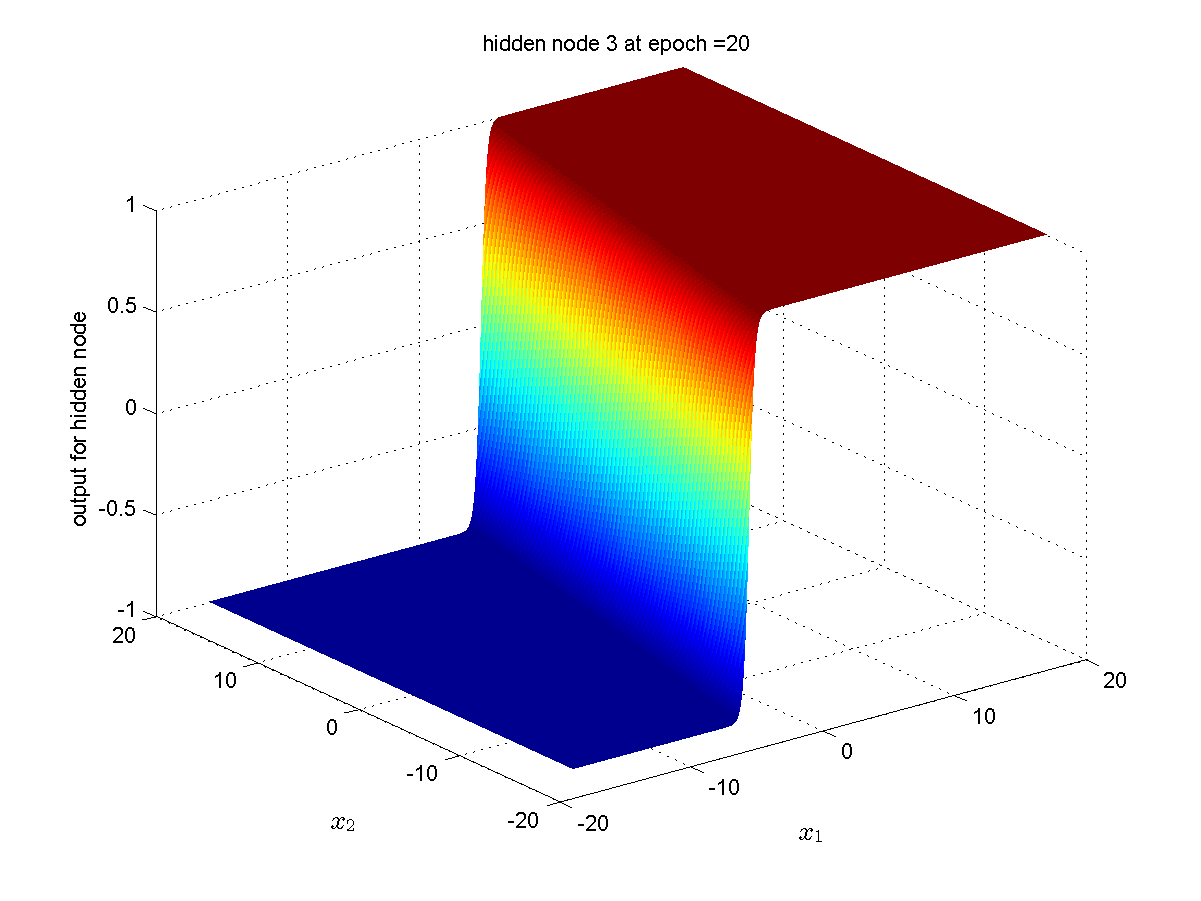
\includegraphics[width=.8\linewidth]{Classification/linearlySeparable/h20_3}
  
\end{subfigure}
\caption{Epoch 20 hidden nodes 1,2,3}
\end{figure}

\begin{figure}
\begin{subfigure}{.3\textwidth}
  \centering
  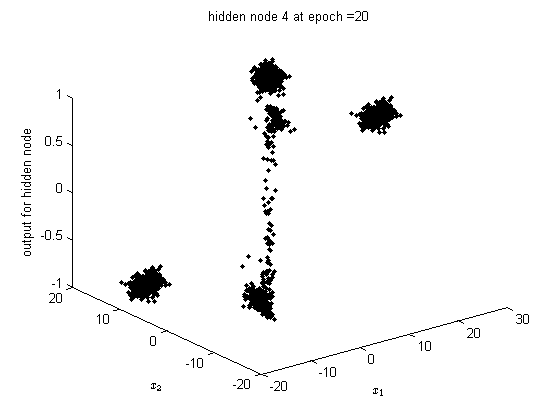
\includegraphics[width=.8\linewidth]{Classification/linearlySeparable/h20_4}
 
\end{subfigure}%
\begin{subfigure}{.3\textwidth}
  \centering
  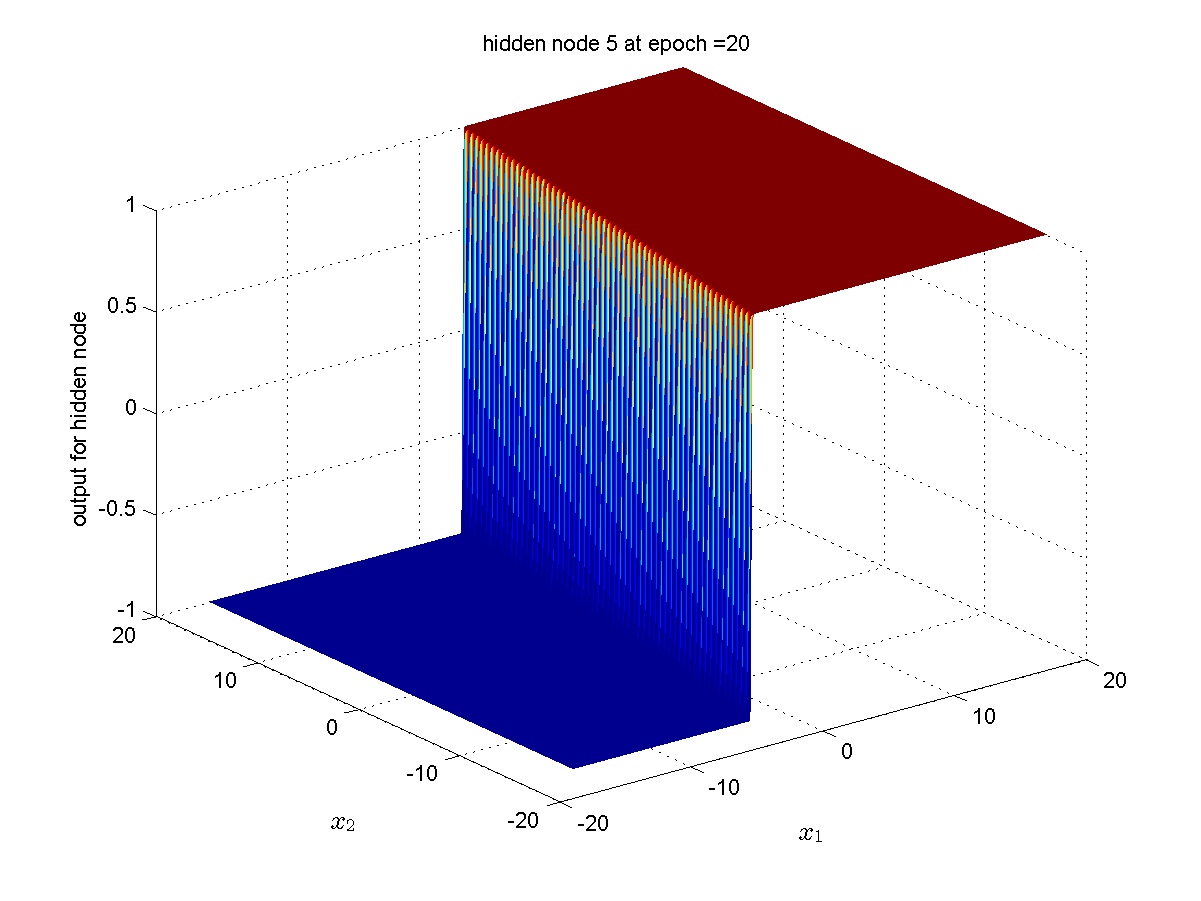
\includegraphics[width=.8\linewidth]{Classification/linearlySeparable/h20_5}
  
\end{subfigure}
\begin{subfigure}{.3\textwidth}
  \centering
  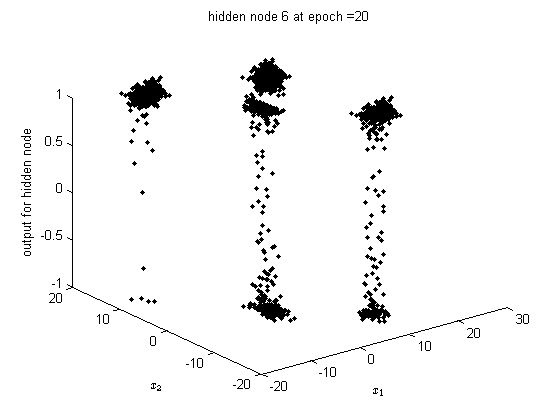
\includegraphics[width=.8\linewidth]{Classification/linearlySeparable/h20_6}
  
\end{subfigure}
\caption{Epoch 20 hidden nodes 4,5,6}
\end{figure}

\begin{figure}
\begin{subfigure}{.3\textwidth}
  \centering
  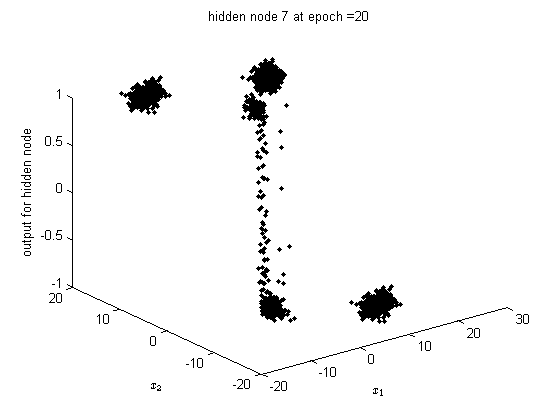
\includegraphics[width=.8\linewidth]{Classification/linearlySeparable/h20_7}
 
\end{subfigure}%
\begin{subfigure}{.3\textwidth}
  \centering
  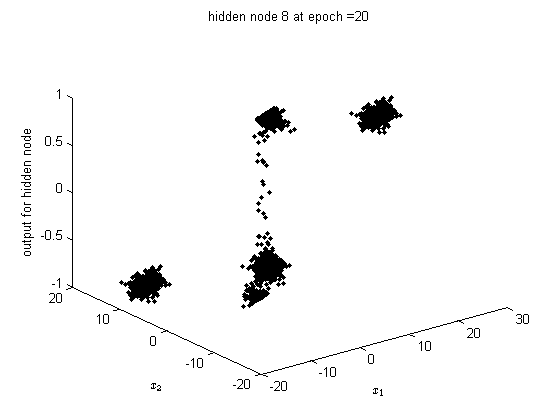
\includegraphics[width=.8\linewidth]{Classification/linearlySeparable/h20_8}
  
\end{subfigure}
\begin{subfigure}{.3\textwidth}
  \centering
  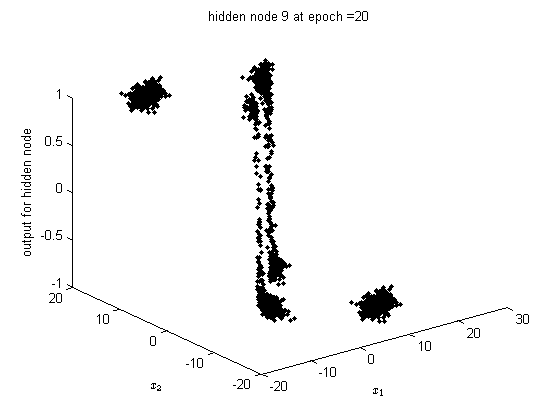
\includegraphics[width=.8\linewidth]{Classification/linearlySeparable/h20_9}
  
\end{subfigure}
\caption{Epoch 20 hidden nodes 7,8,9}
\end{figure}
We can notice the clear S shaped curves that appear out of the hidden layer in these plots. Also note that the difference between epochs 5 and 20 is less than that between 1 and 5 as expected.
\newpage
Comparison --
\end{flushleft}

\subsubsection{Non-linearly Separable Dataset}
\begin{flushleft}

In this dataset, we are given a 2 class problem, where every pair of classes is non-linearly separable, i.e the 2 classes can be separated by a non-linear decision boundary. Here, we are required to compare the performance of Bayes classifier and MLFFNN.
The input data is as shown in the figure below. \\[10pt]

\end{flushleft}

\begin{figure}[H]
\centering
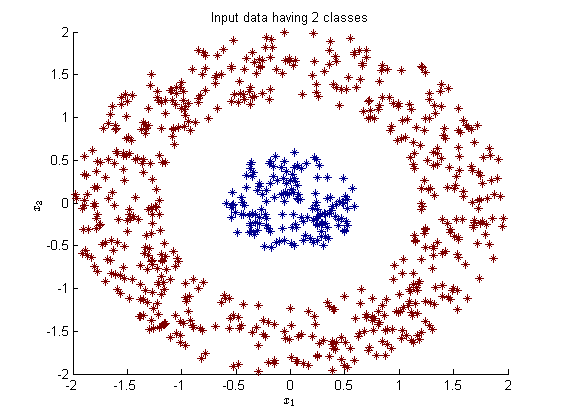
\includegraphics[width=\linewidth]{Classification/nonlinearlySeparable/input_data.png}
\caption{Given dataset}
\end{figure}


\textbf{Bayes classifier :}  \\[10pt]
\begin{flushleft}

The Gaussian mixture model was used to model the class conditional densities of each class. Unlike the previous data, we can see the need to use more than one component in the GMM used to model each of the classes. Hence, we need to choose the appropriate number of Gaussian components to represent each class.
\\[10pt]

For this purpose, we adopt an unsupervised approach. We use the Bayesian Information Criterion (BIC), which provides a trade-off between the likelihood of the data and the model complexity.

\[ \mathrm{BIC} = {-2 \cdot \ln{\hat L} + k \cdot \ln(n)}. \ \]

where $\hat L$ is the maximized likelihood, $k$ is the no. of parameters, and $n$ the number of data points. The model with the lowest BIC value is expected to be the best one.


Based on this criterion, we obtained 3 Gaussian components for class 1 (inside region) and 5 Gaussian components for class 2. The Gaussian contours obtained for each of the classes are shown in the figures below.



\end{flushleft}


\begin{figure}[H]
\centering
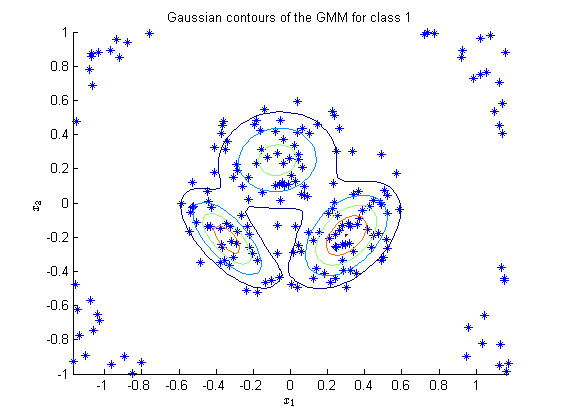
\includegraphics[width=\linewidth]{Classification/nonlinearlySeparable/gmm_1.png}
\caption{Gaussian contours for class 1}
\end{figure}



\begin{figure}[H]
\centering
\includegraphics[width=\linewidth]{Classification/nonlinearlySeparable/gmm_2.png}
\caption{Gaussian contours for class 2}
\end{figure}

\begin{flushleft}

From these contours, we can validate the appropriateness of the metric used, as the gaussian components accurately model the inter-class variability.

The results obtained are shown below : \\[10pt]

\textbf{Train} : \\[10pt]

\begin{tabular}{|c|c|}  \hline 150 & 0\\ \hline 0 & 600 \\ \hline \end{tabular} \\[10pt]

\textbf{Validation} : \\[10pt]

\begin{tabular}{|c|c|} \hline 90 & 0\\ \hline 0 & 360 \\ \hline \end{tabular} \\[10pt]


\textbf{Test} : \\[10pt]
\begin{tabular}{|c|c|}  \hline 60  & 0\\ \hline 0 & 240 \\ \hline \end{tabular} \\[10pt]

\begin{flushleft}
As expected, since the Gaussian adequately model the distributions of the 2 nonlinearly separable classes, we get 100 \% accuracy on all 3 sets.

The decision region plot separating the 2 classes is shown below :

\end{flushleft}

\end{flushleft}

\begin{figure}[H]
\centering
\includegraphics[width=\linewidth]{Classification/nonlinearlySeparable/decn_region_bayes.png}
\caption{Decision region plot}
\end{figure}



\begin{flushleft}
\textbf{MLFFNN} \\[10pt]
Here again, as in the previous dataset, we use a neural network with 1 hidden layer, for which the number of nodes is estimated using cross validation on the given validation dataset.

For the best performance on the validation data, we get ?? nodes in the hidden layer. For this configuration, the results obtained are shown below :

\end{flushleft}
% Confusion matrices %

\begin{flushleft}
The decision region plot obtained is shown below in Figure ..

The outputs of hidden and output nodes are shown below ..

\end{flushleft}


Comparison --



\subsubsection{Overlapping classes Dataset}
\begin{flushleft}
In this dataset, we are given a 2 class problem, where every pair of classes is linearly non separable, i.e the most of the points can be separated by a linear decision boundary but a few points of each class lie on either side of the boundary. Here, we are required to compare the performance of Bayes classifier and MLFFNN.

The input data is as shown in the figure below. \\[10pt]
\end{flushleft}

\begin{figure}[H]
\centering
\includegraphics[width=\linewidth]{Classification/overlapping/input_data.png}
\caption{Given dataset}
\end{figure}


\begin{flushleft}

\textbf{Bayes Classifier :} \\[10pt]


The Gaussian mixture model was used to model the class conditional densities of each class. In this dataset, we observe that using only Gaussian is sufficient to model the points in each class. This hypothesis was however verified using the BIC criterion. The gaussian contours obtained for the classes are shown in the figure below.


\end{flushleft}

\begin{figure}[H]
\centering
\includegraphics[width=\linewidth]{Classification/overlapping/gmm.png}
\caption{Gaussian contours of the 4 classes}
\end{figure}

\begin{flushleft}

The results obtained are shown below : \\[10pt]

\textbf{Train} : \\[10pt]
\begin{tabular}{|c|c|c|c|} \hline 216 & 7 & 19 & 8\\ \hline 9 & 234 & 4 & 3\\ \hline 24 & 1 & 225 & 0\\ \hline 2 & 4 & 0 & 244 \\ \hline \end{tabular} \\[10pt]


\textbf{Validation} : \\[10pt]

\begin{tabular}{|c|c|c|c|} \hline 134 & 2 & 6 & 8\\ \hline 7 & 139 & 2 & 2\\ \hline 12 & 1 & 137 & 0\\ \hline  4 & 5 & 0 & 141 \\ \hline \end{tabular} \\[10pt]




\textbf{Test}: \\[10pt]


\begin{tabular}{|c|c|c|c|} \hline 90 & 1 & 7 & 2\\ \hline 7 & 88 & 4 & 1\\ \hline 14 & 3 & 83 & 0\\ \hline 2 & 0 & 0 & 98  \\ \hline \end{tabular} \\[10pt]



The decision region plot obtained is shown below :

\end{flushleft}

\begin{figure}[H]
\centering
\includegraphics[width=\linewidth]{Classification/overlapping/decn_region_bayes.png}
\caption{Decision region separating the 4 classes}
\end{figure}



\begin{flushleft}
\textbf{MLFFNN} \\[10pt]
Here again, as in the previous dataset, we use a neural network with 1 hidden layer, for which the number of nodes is estimated using cross validation on the given validation dataset.

For the best performance on the validation data, we get ?? nodes in the hidden layer. For this configuration, the results obtained are shown below :

\end{flushleft}
% Confusion matrices %

\begin{flushleft}
The decision region plot obtained is shown below in Figure ..

The outputs of hidden and output nodes are shown below ..

\end{flushleft}





\subsection{Dataset 2 - Image dataset}
In this dataset, we are given a set of images and are required to classify them according to the labels, which are  :


\begin{enumerate}

\item    light-house

\item    treadmill

\item    ladder

\item    leopards

\item    faces-easy


\end{enumerate}

The features extracted from the image are Color Histogram Features which give rise to $16 \times 3 = 48$ features.  We are required to compare the Bayes classifier and neural network classifier on this dataset.


\begin{flushleft}

\textbf{Bayes classifier :} \\[10pt]

In this case, as the number of dimensions is high, we chose to model the gaussians in the  mixture model with a diagonal covariance matrix. This was because the number of parameters needed to be estimated for each gaussian would be at least 2350, which much larger than the number of training examples we have for each class. We also use a small regularization parameter which is added to the covariance matrix to prevent singularity, as the features present were correlated. \\[10pt]


To find the number of gaussian components to use in the class conditional densities of each class, we used the performance (MSE) on the validation data to estimate the best number of components. The plot showing the variation of mis-classification error with the number of gaussian components is shown below :

\end{flushleft}

\begin{figure}[H]
\centering
\includegraphics[width=\linewidth]{Classification/images/MisClassFraction.png}
\caption{Plot to find number of gaussian components}
\end{figure}
\begin{flushleft}

Here, we get 5 mixture components for each gaussian. 

The performance results obtained on splitting the data into train, validation and test are shown below :

\textbf{Train} : \\[10pt]


\begin{tabular}{|c|c|c|c|c|} \hline 54 & 20 & 35 & 0 & 5\\ \hline 4 & 58 & 12 & 1 & 13\\ \hline 2 & 32 & 88 & 0 & 20\\ \hline 0 & 0 & 0 & 114 & 0\\ \hline 0 & 4 & 3 & 0 & 254 \\ \hline \end{tabular}\\[10pt]

Train Accuracy : 79 \% \\[10pt]

\textbf{Validation} :  \\[10pt]
\begin{tabular}{|c|c|c|c|c|} \hline 11 & 7 & 14 & 0 & 7\\ \hline 2 & 21 & 4 & 0 & 2\\ \hline 5 & 12 & 23 & 0 & 8\\ \hline 0 & 0 & 0 & 39 & 0\\ \hline 1 & 9 & 3 & 0 & 74 \\ \hline \end{tabular}\\[10pt]

Validation Accuracy : 69.42  \% \\[10pt]
\textbf{Test} :  \\[10pt]
\begin{tabular}{|c|c|c|c|c|}  \hline 9 & 7 & 17 & 0 & 4\\ \hline 2 & 19 & 7 & 0 & 2\\ \hline 9 & 13 & 17 & 0 & 9\\ \hline 0 & 0 & 0 & 37 & 0\\ \hline 0 & 3 & 2 & 0 & 82 \\ \hline \end{tabular}\\[10pt]

Test Accuracy : 68.62 \% \\[10pt]


We observe that the accuracy obtained here, is quite less. One of the ways this can be improved is by considering different number of gaussian mixture components for each class.


\textbf{MLFFNN :}

\end{flushleft}

\section{Regression task}
In this task, we are given the same 2 datasets as the first assignment. In this assignment, we are required to use the MLFFNN and RBFNN models for the purpose of function approximation, specifically curve fitting and surface fitting in datasets 1 and 2 respectively.


\subsection{Dataset 1 (Univariate)}
\begin{flushleft}
Here, we are required to do curve fitting of the function $e^{cos(2 \pi x)}$.
\end{flushleft}

\textbf{MLFFNN :}

\textbf{Generalized RBF model :}

\subsection{Dataset 2 (Bivariate)}




%\begin{figure}[H]
%
%\begin{subfigure}{.5\textwidth}
%\centering
%\includegraphics[width=\linewidth]{D2/Varyinglambda_N1000M1000lambda1e-06}
%\caption{$\lambda$ = $10^{-6}$}
%\end{subfigure}
%\begin{subfigure}{.5\textwidth}
%\includegraphics[width=\linewidth]{D2/Varyinglambda_N1000M1000lambda0_01}
%\caption{$\lambda$ = 0.01}
%\end{subfigure}
%
%\end{figure}



\end{document}
